% Build: pdflatex main && bibtex main && pdflatex main && pdflatex main
\documentclass[11pt]{article}
\usepackage[margin=1in]{geometry}
\usepackage{times}
\usepackage{booktabs}
\usepackage{amsmath,amssymb}
\usepackage{graphicx}
\usepackage{caption}
\usepackage{array}
\usepackage{url}
\usepackage[colorlinks=true,linkcolor=blue,citecolor=blue,urlcolor=blue]{hyperref}
\captionsetup{font=small,labelfont=bf}
\frenchspacing
\setlength{\parskip}{1pt}

% Companion repository.
\newcommand{\repourl}{https://github.com/bro789/rlvr-control-group-audit-icassp2027}

\title{Something Simpler Wins, But Not Always the Same One:\\
Auditing RLVR Control Groups Across Three Backbone Scales\\[6pt]
\large Extended version: complete per-group statistics, aggregator sensitivity\\
and a selection-bias audit of the decision rule}

\author{Keyi Li \and Yihao He \and Quanyi Li \and Guanghui Liu \and Xiaoyu Lu \and
Linying Jiang\thanks{Corresponding author: \texttt{jiangly@swc.neu.edu.cn}}\\[4pt]
\normalsize Software College, Northeastern University, Shenyang, China}

\date{\today}

\begin{document}
\maketitle

\begin{abstract}
Reinforcement learning with verifiable rewards (RLVR) is evaluated against a
remarkably uniform control group: the base model, matched supervised
fine-tuning, sometimes rejection-sampling SFT. All of these are learning arms
whose accuracy grows with the demonstration budget. We pre-registered, before
the second task was run, a decision rule comparing GRPO against the
\emph{maximum} over a four-arm control group, one arm of which is a
deterministic symbolic solver that does not learn. Across two program-annotated
financial QA tasks and three backbones spanning $14\times$ in scale, all 17
frozen-test effect sizes are negative, from $-1.06$ to $-16.42$ points. The
mechanism is a moving baseline: the solver attains the maximum at 0.5B and 1B
because it is flat in the demonstration budget, while at 7B it falls 15 points
behind and continued SFT takes its place. Ablations, a verifier-hacking audit
over 57{,}517 positive-reward samples and a KL sweep all leave the sign
unchanged.

\medskip
\noindent
\textbf{One boundary, found by us and reported here.} Config~3 was included to
answer ``your models are too small.'' It cannot. Re-running its
smallest-margin cell at ten times the prompt coverage reverses it decisively:
GRPO reaches $87.23\%$ and $86.88\%$ against continued SFT's $80.50\%$
($\Delta = +6.74$, $+6.38$; McNemar $p = 0.0013$, $0.0029$), which clears this
paper's own Go threshold. At the \emph{registered} budget nothing changes, and a
run that fixes the degeneracy we diagnose lands at $+1.06$ with an interval of
$[-2.13, +4.26]$ --- statistically the same place as the original $-1.06$. So
the 7B result marks a \emph{budget} boundary, not a capability one, and the
quantitative core of this paper is the 11 groups at 0.5B and 1B. Details in
Appendix~\ref{app:followup}.

\medskip
\noindent
The rest of this extended version adds the material a four-page paper cannot
carry, and it is deliberately two-sided. In our favour: the $\max$ in the
decision rule is
\emph{not} responsible for the negative sign---a cross-fitted estimator that
selects the control arm on one half of the test set and scores it on the other
still yields a negative $\Delta$ in 17 of 17 groups (mean $-4.18$ against a
naive $-4.44$), and the bootstrap selection bias never exceeds $0.47$ points;
the inference-time sampling arm that is usually proposed as the missing
baseline is not deployable on these tasks, and even its oracle upper bound
(pass@16) loses to the solver at three of four operating points. Against us:
under Holm correction across all 17 groups only \textbf{2} are significant, the
per-group bootstrap intervals exclude zero in only 5, and \textbf{no GRPO run
completed even one epoch} over its prompt pool ($0.10$--$0.79$ epochs; at 7B
roughly $10\%$). We report all of it, with every number regenerated from the
stored per-item outcome vectors by a single script.
\end{abstract}

\tableofcontents
\bigskip

\section{Introduction}

Reinforcement learning with verifiable rewards (RLVR) has become the default
recipe for improving symbolic reasoning: sample programs, execute them, reward
the correct ones, optimize with a policy-gradient method such as
GRPO~\cite{grpo2024}. Reported gains are large and consistent~\cite{deepseekr1}.

What those gains are measured against is remarkably uniform. Across the
empirical RLVR literature the control group consists of \emph{learning} arms:
the un-tuned base model, a matched supervised fine-tuning (SFT) run on the same
demonstrations, and---in the more careful papers---rejection-sampling
SFT~\cite{rft2023,restem2023}. Every one of these consumes the demonstration
budget and improves as it grows. A fourth option is almost never present: a
deterministic, non-learning symbolic solver. For program-annotated numerical
reasoning benchmarks such as FinQA~\cite{finqa2021} or
TAT-QA~\cite{tatqa2021}, where answers are short arithmetic programs over a
table, such a solver is not exotic---it is the classical approach the neural
pipeline replaced.

This paper asks whether that omission changes conclusions, and finds something
more general than expected.

\paragraph{The observation that starts it.}
With two demonstrations on CodeTAT-QA, warm-start SFT reaches $19.0\%$ dev
accuracy and GRPO reaches $72.0\%$---a 53-point gain that, against a
warm-start-only control, is an unambiguous success. A rule-based solver handed
the \emph{same} two demonstrations---and using neither---also reaches $72.0\%$.
On the frozen test
set the three seeds give $\Delta = -2.13$, $-1.42$, $-3.90$ points. The gain
over the learning baseline is real; the conclusion drawn from it is not.

\paragraph{Design.}
We pre-registered---before running anything on the second task---a single
decision quantity:
\begin{equation}
\label{eq:delta}
\Delta(m) = \mathrm{Acc}(\mathrm{GRPO}|W_m) - \max_{a \in \mathcal{B}} \mathrm{Acc}(a),
\end{equation}
with $\mathcal{B} = \{W_m, \text{c-SFT}, \text{RS-SFT}, \text{solver}\}$, all
arms branching from the same warm start $W_m$ trained on the same $m$
demonstrations. Taking a $\max$ over the control group, rather than comparing
against one chosen opponent, is the central design decision: it makes the
comparison impossible to ease by dropping an arm.

\paragraph{Findings.}
We evaluate two tasks and three backbones spanning $14\times$ in scale. All 17
frozen-test groups give negative $\Delta$, from $-1.06$ to $-16.42$ points
(Figure~\ref{fig:delta}). But the interesting structure is in \emph{which} arm
wins:

\begin{itemize}\itemsep2pt
\item At \textbf{0.5B and 1B}, the maximum is attained by the deterministic
solver in every one of 11 groups. Dose-response curves explain why: the solver
is flat in the demonstration budget while every learning arm scales steeply
with it, so the scarce regime is where a non-learning baseline is strongest.
\item At \textbf{7B}, the solver drops 15 points behind and is no longer
competitive---exactly as the ``RLVR gains emerge with backbone capability''
account predicts. $\Delta$ stays negative in all six groups anyway, because the
winning arm becomes \textbf{continued SFT}: the most elementary baseline in the
set, and one that appears in essentially every RLVR paper.
\end{itemize}

So the finding is not ``a symbolic solver beats RL''---that is a fact about one
scale regime. It is that \emph{at every scale we measured, some simpler method
matched or beat GRPO, but which method that is changes with scale}. A control
group holding only the base model and one matched SFT run misses the solver at
0.5B; a control group designed around the solver misses continued SFT at 7B.
What the evidence demands is breadth of the control group and a $\max$
aggregation over it, not the presence of any particular arm.

\paragraph{Contributions.}
(i) A control-group design for RLVR evaluation---a non-learning arm plus $\max$
aggregation---together with the pre-registered decision rule built on it;
(ii) an execution over two tasks and three backbones in which all 17
frozen-test effect sizes are negative and the identity of the winning baseline
shifts with scale; (iii) three independent observations of dev-selection bias,
each a non-negative $\Delta$ on dev that turns negative on the frozen test.

Section~\ref{sec:statistics} additionally audits the decision rule against the
selection bias it could itself introduce, and finds that it does not account for
the result. We report that as an audit of our own instrument rather than as a
contribution, alongside the per-group statistics---two of seventeen groups
significant under Holm---that the effect sizes actually support.

\paragraph{What we do not claim.}
We do not claim RLVR is ineffective: our GRPO runs beat every learning baseline
at 0.5B, by 35 points at $m{=}2$. We do not claim the solver generalizes---it is
task-specific and its engineering cost is reported in
Section~\ref{subsec:solvercost}. We do not claim the 7B groups establish a
scale effect: at ten times the prompt coverage the smallest-margin 7B cell
reverses to $\Delta = +6.74$ (Appendix~\ref{app:followup}), so Config~3 marks a
budget boundary rather than a capability one. We claim only that an RLVR
conclusion established without a broad control group, a stated budget and a
frozen test set is not trustworthy.

\section{Related Work}
\label{sec:related}

\paragraph{RLVR and its control groups.}
GRPO~\cite{grpo2024} and its descendants~\cite{deepseekr1} optimize against
an executable checker rather than a learned reward model, which removes reward
hacking of the preference-model kind and makes the training signal cheap on
program-annotated tasks. Empirical reports pair RLVR against the base policy
and a matched SFT run; stronger evaluations add rejection-sampling SFT or
iterated self-training~\cite{star2022,rft2023,restem2023}, which use the same
verifier at training time without policy-gradient updates. Every arm in these
control groups is a learning arm whose accuracy grows with the demonstration
budget. Our contribution is not a new algorithm but the observation that adding
one non-learning arm changes the sign of the reported effect.

Recent critical work on R1-Zero-style training has begun to audit the recipe
itself rather than its reported margins. Dr.\ GRPO~\cite{drgrpo2025} identifies
an optimization bias in GRPO's length normalization, and
SimpleRL-Zoo~\cite{simplerlzoo2025} shows how sharply the outcome of zero-RL
training depends on the base model across ten backbones. Both findings concern
what happens \emph{inside} the RL arm. Our question is orthogonal and
complementary: holding the RL arm fixed, what does the control group have to
contain before its reported margin means anything? A paper can adopt Dr.\ GRPO's
unbiased estimator and still report a gain that a non-learning arm erases.

\paragraph{Does RL exceed the base model's reach?}
A parallel line asks whether RLVR expands a model's capability or merely
sharpens its sampling distribution, e.g.\ by comparing pass@$k$ before and
after RL~\cite{yue2025limit} or by auditing where reported gains come
from~\cite{sober2025}. That question is about the policy; ours is about the
comparison. The two can agree in direction while differing in what would refute
them: our claim would be refuted by a strong solver that still loses to GRPO,
not by a demonstration that RL narrows the output distribution.

\paragraph{Weak baselines as a source of illusory progress.}
The stance we adopt has an explicit lineage, which the conference version of
this paper invoked without citing. In recommendation, Ferrari Dacrema et
al.~\cite{dacrema2019} reproduced only 7 of 18 recent neural methods and found
6 of those 7 beaten by properly tuned classical baselines. In deep metric
learning, Musgrave et al.~\cite{musgrave2020} found a decade of reported gains
largely attributable to experimental protocol. In neural
retrieval,~\cite{lin2018hype} made the same argument about comparisons against
untuned BM25. Deep RL has its own version of the problem: Henderson et
al.~\cite{henderson2018matters} showed that reported margins can be smaller
than the variation induced by random seeds, and Agarwal et
al.~\cite{agarwal2021precipice} showed that point estimates over few runs
routinely misrepresent aggregate performance.

We add two elements specific to RLVR. First, the baseline we restore is
\emph{non-learning}, so---unlike a tuned BM25 or a tuned matrix
factorization---it cannot be strengthened by spending more of the demonstration
budget, which is what makes it bind precisely in the scarce regime where RLVR
is argued to be valuable. Second, the decision rule is fixed by
pre-registration before the second task is run, so the comparison cannot be
retrofitted to the result.

\paragraph{Test-set reuse and selection.}
Our design reserves a frozen test set and evaluates each arm on it exactly
once, which is the operational form of a long-standing concern about adaptive
analysis. Dwork et al.~\cite{dwork2015holdout} give the theory of how repeated
querying of a holdout destroys its validity; Recht et
al.~\cite{recht2019} give the empirical counterpart on ImageNet. Our
Section~\ref{sec:results} reports three instances of the same phenomenon inside
a single study, and Section~\ref{sec:statistics} audits our own decision
quantity for the selection bias it could itself introduce. For multiple
comparisons we use Holm's sequentially rejective procedure~\cite{holm1979},
and for the interpretation of non-significant per-group results we follow
Card et al.~\cite{card2020power} on the power that small NLP test sets actually
afford.

\paragraph{Symbolic and program-based numerical reasoning.}
Program-of-Thought~\cite{pot2022} and PAL~\cite{pal2023} delegate arithmetic
to an interpreter, which is what makes verifiable rewards natural on these
tasks. The same property makes a purely deterministic solver feasible:
FinQA~\cite{finqa2021}, ConvFinQA~\cite{convfinqa2022} and
TAT-QA~\cite{tatqa2021} annotate answers with short executable programs over
semi-structured tables, and BizBench~\cite{bizbench2024} packages
CodeFinQA and CodeTAT-QA in that form.

The observation that policy gradients can be trained against an executable
checker on exactly this kind of table-program task is not new, and predates
RLVR by most of a decade. Neural Symbolic Machines~\cite{nsm2017} trained a
sequence-to-program model against a Lisp interpreter with REINFORCE under weak
supervision; MAPO~\cite{mapo2018} added a memory buffer of verified
trajectories to reduce gradient variance, on WikiTableQuestions~\cite{wtq2015}
and WikiSQL. The control-group problem we describe is visible in that
literature too, where deterministic semantic parsers remained competitive
baselines. Later, Binder~\cite{binder2023} reached state of the art on the same
table-QA benchmarks with no training at all, by binding a language model into a
symbolic program---the strongest existing evidence that on table-program tasks
the non-learning route is a serious competitor rather than a straw arm. Our
solver is a port of classical label-alignment and operator-template machinery,
not a novel method, which is exactly why its omission from RLVR control groups
is hard to justify.

\paragraph{Pre-registration and frozen evaluation.}
Pre-registration, held-out test sets touched once, and explicit deviation logs
are standard in fields where negative results must be credible. They are rare
in ML practice but disproportionately valuable for a paper whose main result is
a null: without a decision rule fixed in advance, a reader cannot distinguish
``the effect was absent'' from ``the analysis was run until the effect was
absent.'' Appendix~\ref{app:reproduce} states what was frozen when, which
comparisons are confirmatory and which are exploratory, and where the full
protocol and its logged deviations can be read.

\section{Experimental Setup}
\label{sec:setup}

\paragraph{Tasks and models.}
We use three configurations built on BizBench~\cite{bizbench2024}, chosen so
that the dataset family, the model family, the backbone scale, and the strength
of the deterministic baseline all vary:

\begin{itemize}\itemsep2pt
\item \textbf{Config~1}: CodeTAT-QA $\times$ Qwen2.5-0.5B-Instruct. Context is a
JSON table; gold programs index cells as \texttt{df["col"]["row"]}. 2846 clean
training items, 400 held out as dev (all selection uses a fixed 200-item subset
of it), frozen test $n{=}282$.
\item \textbf{Config~2}: CodeFinQA $\times$ Llama-3.2-1B-Instruct. Context is
narrative financial-report text with embedded tables; gold programs inline the
numbers. 4035 clean training items, 400 dev (same 200-item convention), frozen
test $n{=}664$.
\item \textbf{Config~3}: CodeTAT-QA $\times$ Qwen2.5-7B-Instruct. Identical
task, data splits, budgets, and protocol to Config~1 with a $14\times$ larger
backbone; this is the scale probe of Section~\ref{sec:scale}.
\end{itemize}

An item is \emph{clean} if its gold program executes to its gold answer under
our verifier: $2846/2856 = 99.65\%$ for CodeTAT-QA and $4035/4668 = 86.4\%$ for
CodeFinQA. The ten CodeTAT-QA failures were inspected individually and are
dataset defects (a final line not assigned to \texttt{answer}, or a
comprehension with no bare binary operation), not adaptation artifacts.

\paragraph{Demonstration budgets.}
Nested subsets are drawn from the clean pool, so a smaller budget is always a
prefix of a larger one. Config~1 uses
$m \in \{0,1,2,4,8,16,64,256,1024,2446\}$ and Config~2 uses
$m \in \{0,16,64,128,256,1024,3635\}$, where the largest value is the full
pool. Three independent subset seeds are drawn per configuration; every arm at
a given $(m, \text{seed})$ sees exactly the same $m$ demonstrations.

\paragraph{Pre-registration.}
The decision quantity in Eq.~\eqref{eq:delta}, the gate criteria, the budget
selection rule, and the verdict vocabulary were frozen before any training or
evaluation run on the second task. The protocol also fixed, in advance, how a
result contrary to our expectation would be handled: \emph{if the solver is
strong and GRPO nevertheless wins, report it as such, and do not weaken the
solver to recover the original narrative}. Both outcomes were accepted at
freeze time. The solver's construction was likewise constrained ex ante to a
``good-faith maximum effort'' clause forbidding template pruning or threshold
tuning in response to intermediate results.

\paragraph{Budget selection.}
Two operating points are chosen per configuration from the warm-start dose
curve using the pre-registered bands: $m_L$ is the smallest budget landing in
$[5\%, 20\%]$ dev accuracy and $m_H$ the smallest in $[25\%, 45\%]$. This
yields $m_L{=}2, m_H{=}64$ for Config~1 and $m_L{=}128, m_H{=}256$ for
Config~2. When the initial grid left the low band empty, additional budgets
were run rather than reinterpreting the band---this is one of the logged
deviations.

\paragraph{Leakage control.}
We assert disjointness of dev, demonstration pool, and test, and verify before
each solver run that its retrieval library does not intersect dev. The frozen
test set is untouched during training, checkpoint selection, and budget
selection; every arm is evaluated on it exactly once, at the checkpoint already
selected on dev.

\paragraph{Deviations.}
Minor protocol adjustments (e.g., adding intermediate budget points when initial grids left required bands empty) were logged alongside their influence direction.

\section{Five Arms and the Decision Rule}
\label{sec:method}

\begin{figure}[t]
\centering
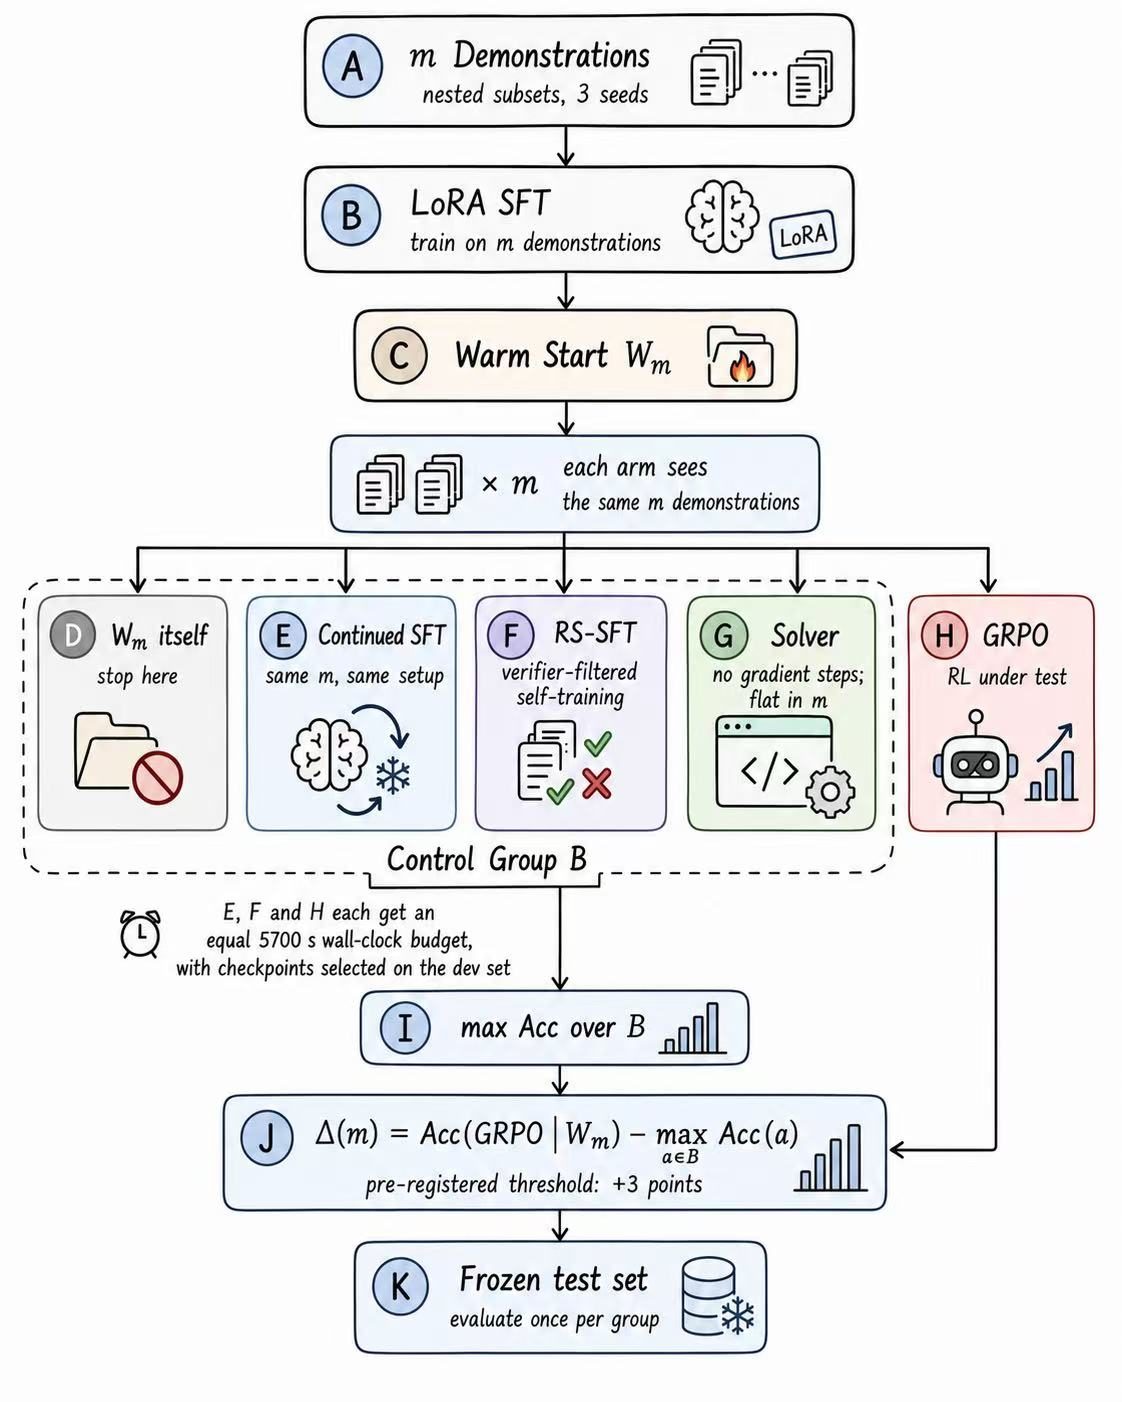
\includegraphics[width=0.92\textwidth]{figs/fig1_design.jpg}
\caption{The five arms and the decision rule. Every arm branches from the same
warm start $W_m$ and sees the same $m$ demonstrations, so the comparison is
about what to do next with a fixed budget. $\Delta$ takes the \emph{maximum}
over the four-arm control group $\mathcal{B}$.}
\label{fig:design}
\end{figure}

All arms branch from a common warm start $W_m$: a LoRA SFT run on the $m$
demonstrations of that budget and seed. This makes the comparison about
\emph{what to do next with the same $m$ demonstrations}, not about different
amounts of supervision.

\paragraph{The four baseline arms.}
$W_m$ itself is the starting point. \textbf{Continued SFT} keeps imitating the
same $m$ demonstrations under the same optimizer settings. \textbf{RS-SFT}
samples from the current policy on pool questions whose gold programs are
\emph{not} revealed, keeps verifier-accepted trajectories, and fine-tunes on
them, iterating. \textbf{The solver} is a deterministic program: it parses the
table, aligns question tokens to row and column labels through a cascade
(exact $\rightarrow$ normalized $\rightarrow$ fuzzy $\rightarrow$ year/numeric
$\rightarrow$ synonym), classifies the arithmetic intent, and emits a program.
Its \emph{scarce} variant---the protocol-compliant one---may retrieve from
exactly the $m$ gold programs of that budget, matching the demonstration
budget of the learning arms. A \emph{full} variant with access to the whole
pool is computed for diagnosis only and never enters $\mathcal{B}$.

\paragraph{The tested arm.}
GRPO~\cite{grpo2024} starts from the same $W_m$ and trains on pool questions
with the verifier as reward, under a wall-clock budget matched to continued SFT
and RS-SFT (Config~1: GRPO 5701--5728\,s, c-SFT 5703--5707\,s at $m{=}64$,
RS-SFT 4561--5815\,s). We note one budget asymmetry in the opposite direction
of our conclusion: at $m{=}2$ in Config~1, continued SFT converged in
2579--3196\,s against GRPO's 5701--5703\,s, so GRPO received more compute than
the baseline it is compared with.

\paragraph{Implementation and compute.}
All runs use PyTorch 2.10, \texttt{transformers} 4.57, \texttt{peft} 0.19 and
\texttt{trl} 1.8 on a single NVIDIA RTX A6000 (48\,GB) per run. All generation
uses HuggingFace \texttt{generate} throughout: we tested swapping in vLLM and
found it shifts accuracy by $3.00$ points---the same magnitude as our Go
threshold, and in no systematic direction---so the substitution was rejected
(Appendix~\ref{subsec:enginegate}). Every arm
trains a LoRA adapter ($r{=}16$, $\alpha{=}32$, dropout $0$) at learning rate
$10^{-5}$; GRPO uses 8 generations per prompt, KL coefficient $\beta{=}0.04$,
temperature $1.0$, top-$p$ $0.95$, and effective batch 64 (per-device 16,
accumulation 4), reduced to per-device 4 with accumulation 16 at 7B to fit the
card. Each arm is capped at 5700\,s of wall clock, enforced at step boundaries, so
runs may overshoot by one step. Checkpoints are selected on
dev; the test set is evaluated once per group. Section~\ref{sec:analysis}
reports the sweep over $\beta$, the only hyperparameter we
varied after the protocol was fixed.

\paragraph{Decision rule.}
$\Delta(m)$ follows Eq.~\eqref{eq:delta}. Comparison uses integer counts,
$k_{\text{GRPO}} - \max_a k_a \geq \lceil 0.03n \rceil$, to avoid
floating-point boundary effects at the $+3$-point Go threshold. Per-item
agreement is tested with McNemar and corrected with Holm.
Only ``GRPO vs.\ the strongest non-RL arm'' is confirmatory; everything else is
descriptive.

Where the threshold comes from matters for reading a null result, so we state it
rather than assert it. It was fixed between two anchors. The upper one is the
published literature. In the RLVR-for-finance papers we could compare against,
the gain from adding RL on top of SFT, measured on program-annotated financial
QA, runs from $-2.56$ to $+4.0$ points: Fin-R1 reports $+3.0$ on FinQA and
$+4.0$ on ConvFinQA~\cite{finr1_2025}, Fino1 $+1.25$ on
FinQA~\cite{fino1_2025}, and DianJin-R1 $-2.56$ on
FinQA~\cite{dianjinr1_2025}. A bar at five points would therefore have meant
``better than anything published on this task family.'' We restrict the
comparison to program-annotated QA deliberately and note what that excludes: the
one published figure we found that reaches five rather than falling below it is
Fin-R1's $+5.0$ on a benchmark that is not program synthesis. Within the task
family this paper studies, nothing published clears the bar. The lower anchor is
measurement resolution: we estimated single-seed
standard error at three to five points, which makes $+3$ the floor of what this
design can distinguish from seed noise at all. We set the Go criterion at the
lower anchor, $+3$, which is the more permissive of the two.

Because $+3$ therefore sits \emph{inside} the noise band of any single run, the
protocol never let it stand alone. A Go verdict additionally requires that at
least two of the three seeds in a cell be positive, that GRPO beat RS-SFT rather
than only plain SFT, and that the verifier-hacking audit be clean; and an effect
anywhere between two and five points, or one whose seeds disagree in sign, is
declared \textsc{inconclusive} and sent back for two further seeds rather than
adjudicated. The evidence this study rests on is accordingly agreement across
seeds and cells rather than per-group significance---which was the design, not a
retreat, as Section~\ref{sec:statistics} quantifies.

\paragraph{Solver cost.}
The solver is task-specific engineering, requiring roughly 440 new lines of
adaptation code on top of a reusable symbolic execution core. We report this
because the fair reading of our result is not ``a small script beats RL'' but
``a few hundred lines of task-specific symbolic code, which this benchmark
family admits by construction, beats RL under scarcity.''

\section{Results}
\label{sec:results}

\begin{figure}[t]
\centering
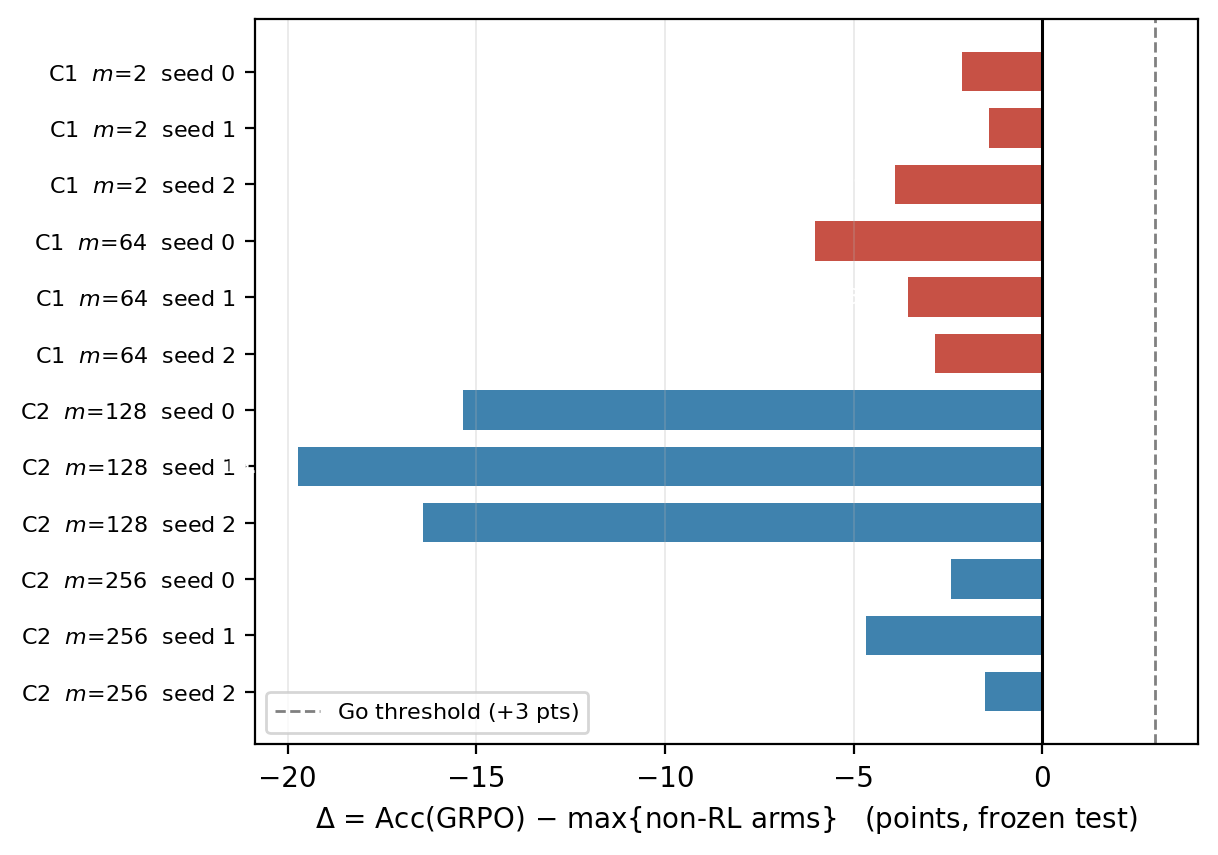
\includegraphics[width=\columnwidth]{figs/F2_delta.png}
\caption{Frozen-test $\Delta$ for all 17 groups, grouped by backbone. Every
value is negative and none approaches the pre-registered $+3$-point Go
threshold (dashed). The arm attaining $\max \mathcal{B}$ is annotated per
band: the solver at 0.5B and 1B, continued SFT at 7B.}
\label{fig:delta}
\end{figure}

\begin{table}[t]
\centering
\small
\setlength{\tabcolsep}{3.2pt}
\caption{Frozen-test accuracy (\%) per arm and $\Delta$ (points) at 0.5B and
1B. The maximum over $\mathcal{B}$ is attained by the solver in all 11 groups.
Config~2 $m{=}128$ seed~1 is excluded: its GRPO run ended with zero positive
reward (Section~\ref{sec:analysis}).}
\label{tab:main}
\begin{tabular}{rr rrrrr r}
\toprule
$m$ & seed & solver & $W_m$ & c-SFT & RS-SFT & GRPO & $\Delta$ \\
\midrule
\multicolumn{8}{l}{\textit{Config~1: CodeTAT-QA $\times$ Qwen2.5-0.5B ($n{=}282$)}} \\
2  & 0 & \textbf{64.54} & 15.60 & 24.47 & 27.66 & 62.41 & $-2.13$ \\
2  & 1 & \textbf{64.54} & 14.54 & 18.09 & 28.01 & 63.12 & $-1.42$ \\
2  & 2 & \textbf{64.54} & 26.60 & 20.57 & 30.50 & 60.64 & $-3.90$ \\
64 & 0 & \textbf{64.54} & 29.43 & 43.62 & 51.06 & 58.51 & $-6.03$ \\
64 & 1 & \textbf{64.54} & 27.66 & 45.39 & 56.03 & 60.99 & $-3.55$ \\
64 & 2 & \textbf{64.54} & 32.62 & 45.74 & 51.42 & 61.70 & $-2.84$ \\
\midrule
\multicolumn{8}{l}{\textit{Config~2: CodeFinQA $\times$ Llama-3.2-1B ($n{=}664$)}} \\
128 & 0 & \textbf{32.38} & 12.05 & 20.18 & 21.84 & 17.02 & $-15.36$ \\
128 & 2 & \textbf{32.53} & 12.65 & 18.83 & 25.00 & 16.11 & $-16.42$ \\
256 & 0 & \textbf{32.38} & 25.60 & 26.36 & 28.92 & 29.97 & $-2.41$ \\
256 & 1 & \textbf{32.83} & 25.75 & 27.11 & 25.90 & 28.16 & $-4.67$ \\
256 & 2 & \textbf{32.08} & 28.16 & 27.41 & 30.27 & 30.57 & $-1.51$ \\
\bottomrule
\end{tabular}
\end{table}

\subsection{Every frozen-test effect size is negative}

Table~\ref{tab:main} and Figure~\ref{fig:delta} give the small-backbone result:
11 groups, $\Delta$ from $-1.42$ to $-16.42$ points, mean $-5.48$. No group
approaches the pre-registered $+3$-point threshold. Adding the six 7B groups of
Section~\ref{sec:scale} gives 17 negative values out of 17, mean $-4.44$.

The two configurations differ in dataset family, model family, and absolute
difficulty---the solver scores $64.54\%$ on Config~1 and $32.08$--$32.83\%$ on
Config~2---yet agree in sign. Config~2 at $m{=}128$ is significant under
McNemar after Holm correction ($p < 0.001$).

One group deserves note for a reason unrelated to $\Delta$: at Config~2
$m{=}128$, GRPO ($16.11$--$17.02\%$) falls below continued SFT
($18.83$--$20.18\%$) and RS-SFT ($21.84$--$25.00\%$). Here the verdict is
negative even without the solver---the learning-only control group already
suffices.

\subsection{Why: the scarce regime is the non-learner's regime}

\begin{figure}[t]
\centering
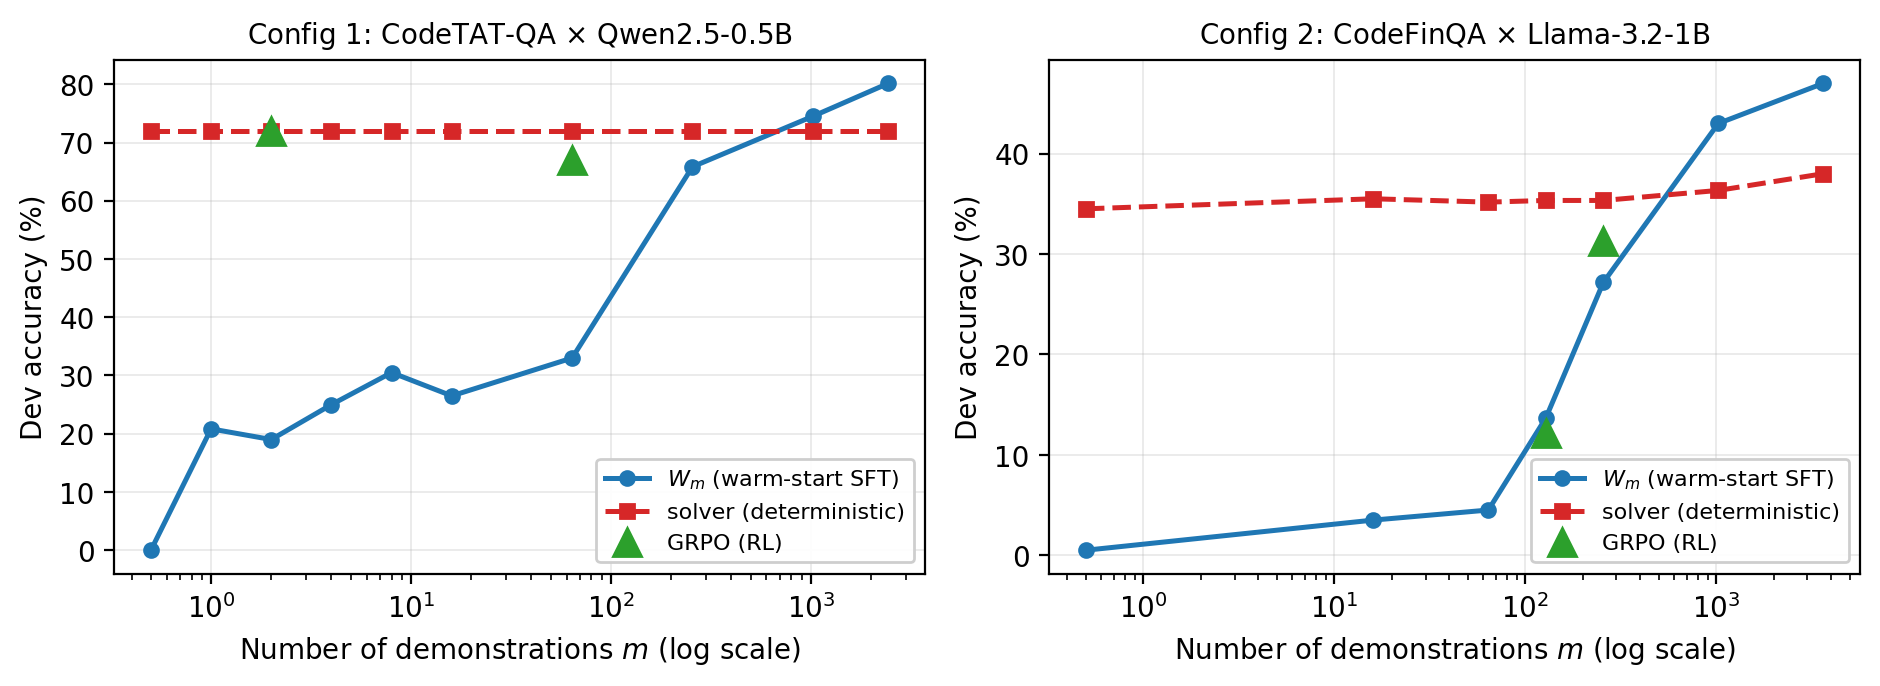
\includegraphics[width=\columnwidth]{figs/F1_dose_curve.png}
\caption{Dose--response curves (dev; three seeds at the operating budgets, one
seed at the diagnostic-only budgets). Learning arms scale with the
demonstration budget; the deterministic solver does not.}
\label{fig:dose}
\end{figure}

Figure~\ref{fig:dose} explains the sign at small scale. Warm-start accuracy in
Config~1 climbs from $0.0\%$ at $m{=}0$ through $19.0\%$ ($m{=}2$), $33.0\%$
($m{=}64$) and $65.8\%$ ($m{=}256$) to $80.2\%$ at the full pool; Config~2
climbs from $0.5\%$ to $47.0\%$. The solver consumes no parameters and learns
nothing: it scores $72.0\%$ at \emph{every one} of Config~1's ten budgets, and
stays within $34.5$--$38.0\%$ across Config~2's seven.

The crossing points matter. In Config~1 the learning curve does not overtake
the solver until $m{=}1024$ ($74.5\%$ vs.\ $72.0\%$); at $m{=}256$ it is still
behind at $65.8\%$. Config~2 crosses near $m{=}1024$ as well ($43.0\%$ vs.\
$36.3\%$). Everything left of that crossing is the demonstration-scarce
regime---the regime in which RLVR is most often argued to be valuable, and in
which a method that ignores demonstrations entirely is hardest to beat.

\subsection{The gain is real; the conclusion is not}

Against a warm-start-only control the same runs look excellent: on dev, GRPO
improves over $W_m$ from $19.0\%$ to $72.0\%$ at $m{=}2$ and from $33.0\%$ to
$67.0\%$ at $m{=}64$. Both would be reported as large positive results. Adding
one non-learning arm to the same comparison turns every frozen-test verdict
negative. RL is doing real work here---it beats every learning baseline by up
to 35 points---but ``does RL beat SFT?'' and ``is RL the best use of this
demonstration budget?'' have different answers.

\subsection{Dev selection bias, observed three times}

On dev, two groups produced non-negative values: Config~1 $m{=}2$ gave
$\Delta = +0.00$, $-0.50$, $+0.50$. The same three groups on the frozen test
gave $-2.13$, $-1.42$, $-3.90$. Two further instances appear later: the
$\beta{=}0$ hyperparameter setting (Section~\ref{sec:analysis}) yields
$+1.50$ on dev and $-2.13$ on test, and the 7B $m{=}2$ seed-2 group yields
$+1.50$ on dev and $-1.77$ on test. In all three, dev favors GRPO and the
frozen test does not.

Since every checkpoint in every arm is selected on dev, the arm whose dev
trajectory fluctuates most gains the most from that selection---and a
policy-gradient run plausibly fluctuates more than a fine-tuning run. We state
this as a candidate mechanism rather than a measured one: three instances
identified after the fact do not establish it, and our stored artifacts support
the per-arm dev-checkpoint variance it predicts only at 7B
(Section~\ref{sec:discussion}). What the three instances do show without
interpretation is the practical point: without a frozen test set we would have
reported non-negative results in three groups and a positive one from the
sweep. All $17 \times 5 = 85$ arm evaluations of the reported groups are
present; nothing in $\mathcal{B}$ is imputed or dropped.


\section{Scale: the winning baseline changes identity}
\label{sec:scale}

The standing objection to everything above is that 0.5B and 1B models are small
enough that RLVR is not expected to help, making the negative result
unsurprising. We test that objection rather than concede it: the same
CodeTAT-QA task, the same protocol, the same two budgets, three seeds, on
Qwen2.5-7B-Instruct.

\begin{table}[t]
\centering
\small
\setlength{\tabcolsep}{3pt}
\caption{Frozen-test accuracy (\%) at 7B, all three seeds. The solver is now
15 points behind and irrelevant; continued SFT attains the maximum in all six
groups and GRPO trails it in all six.}
\label{tab:scale}
\begin{tabular}{rr rrrrr r}
\toprule
$m$ & seed & solver & $W_m$ & c-SFT & RS-SFT & GRPO & $\Delta$ \\
\midrule
2  & 0 & 64.54 & 71.28 & \textbf{79.79} & 75.18 & 76.60 & $-3.19$ \\
2  & 1 & 64.54 & 69.86 & \textbf{77.66} & 76.95 & 74.82 & $-2.84$ \\
2  & 2 & 64.54 & 70.57 & \textbf{76.95} & 74.82 & 75.18 & $-1.77$ \\
64 & 0 & 64.54 & 79.08 & \textbf{81.91} & 80.50 & 79.79 & $-2.13$ \\
64 & 1 & 64.54 & 78.72 & \textbf{80.50} & 80.14 & 79.43 & $-1.06$ \\
64 & 2 & 64.54 & 79.43 & \textbf{85.11} & 81.21 & 80.85 & $-4.26$ \\
\bottomrule
\end{tabular}
\end{table}

Table~\ref{tab:scale} shows the transition. The solver's accuracy is unchanged
by construction---$64.54\%$, the same number as at 0.5B, because it contains no
model---but the learning arms have moved past it. Warm-start SFT on two
demonstrations now reaches $69.86$--$71.28\%$, and every arm at $m{=}64$ is
around $80\%$. The crossing point predicted by the dose-response curves of
Section~\ref{sec:results} is real and lies between 1B and 7B on this task. The
``gains emerge with capability'' account is correct about the solver.

It is not correct about $\Delta$. In all six groups the maximum is attained by
\textbf{continued SFT}---$76.95$--$85.11\%$---and GRPO trails it by $1.06$ to
$4.26$ points (mean $-2.54$). Scaling the backbone $14\times$ replaced the arm
that beats GRPO; it did not produce a setting in which GRPO leads.

\paragraph{What this does to the claim.}
Within the registered budget it generalizes it. Had the solver kept winning at
7B, a reader could reasonably suspect we had over-engineered one baseline for
one regime. Instead the solver exits exactly where the scaling account says it
should, and the arm that replaces it is continued SFT---an arm present in
essentially every RLVR paper, requiring no engineering, and impossible to
characterize as an exotic construction. The methodological requirement that
survives both regimes is not ``include a solver'' but ``make the control group
broad enough that you would notice, and aggregate it with a $\max$.''

\paragraph{But this configuration does not answer the question it was added for,
and we should say so before a reader finds out.}
Config~3 exists to test the objection that 0.5B and 1B are simply too small. It
cannot settle that objection, because at 7B the registered wall-clock budget
buys an order of magnitude less data than it does at 0.5B: $0.13$ epochs over
the prompt pool against $0.53$--$0.79$. We re-ran this section's
smallest-margin cell---$m{=}64$, seed~1, the one most favourable to GRPO---at
ten times the coverage, and it reverses decisively, to $\Delta = +6.74$ and
$+6.38$ across two training seeds, clearing the pre-registered Go threshold
(Appendix~\ref{app:followup}). At the registered budget the result holds,
including under a run that removes the zero-advantage degeneracy we diagnose in
Section~\ref{sec:analysis}. \textbf{What Config~3 demonstrates is therefore a
budget boundary, not a capability one.} We keep it in the paper for that
reason---knowing where a null result stops is worth more than a scale ladder
that does not hold---but the quantitative weight of this study rests on the 11
groups at 0.5B and 1B, not on these six.

\paragraph{Statistical caveats.}
Effect sizes at 7B are smaller than at 0.5B/1B: $-1.06$ to $-4.26$ points on
$n{=}282$ is 3 to 12 items, and the three learning arms lie within a few points
of one another, so which of them attains $\max \mathcal{B}$ is itself sensitive
to sampling noise. Within the registered budget the 7B groups accordingly carry
a qualitative claim---the arm that beats GRPO changes identity, and GRPO is not
that arm in any of the six---rather than an effect size, and past that budget
they do not carry even that. The quantitative result rests on the 11
groups at 0.5B and 1B, where $\max \mathcal{B}$ is attained by a deterministic
solver that leads the nearest learning arm by \emph{at least} $8.5$ points in
Config~1 ($8.51$ to $36.88$ points across the six groups; the quoted figure is
the smallest, not the typical): there the identity of the maximum is not in
question, and no selection over arms enters the estimate.

The largest 7B margin ($-4.26$ points, Config~3 $m{=}64$ seed~2) has an
uncorrected McNemar $p$ of $0.017$. Under the Holm correction this paper
declares across its family of 17 groups, that value becomes $0.254$ and is
\textbf{not} significant; the conference version of this paper quoted the
uncorrected figure alongside a stated Holm procedure, which was inconsistent.
No 7B group is significant after correction. The 7B claim is the qualitative
one stated above, supported by six of six groups agreeing in sign
(Section~\ref{sec:statistics}), and by nothing stronger.

\section{Ruling Out the Obvious Objections}
\label{sec:analysis}

A negative result of this shape invites four specific rebuttals: the solver is
memorizing, its strength is generic to any non-learning method, GRPO's score is
a reward-hacking artifact, and GRPO is simply mistuned. Each is testable; none
survives. We then report the one run we excluded, ask whether our GRPO is
simply under-trained, and state the solver's cost.

\subsection{``The solver is just retrieving gold answers''}

If the solver's accuracy came from copying gold programs out of its retrieval
library, it would be a memorization artifact rather than a baseline. We
decompose it into three variants: \textbf{A} uses only the hand-written rule
path; \textbf{B} uses only retrieval; \textbf{C} is the deployed configuration
(rules first, retrieval as fallback).

\begin{table}[t]
\centering
\small
\caption{Solver ablation (dev, mean of 3 seeds). Retrieval never fires: its
marginal contribution $C-A$ is $+0.00$ points at all ten Config~1 budgets.}
\label{tab:ablation}
\begin{tabular}{rrrr r}
\toprule
$m$ & A: rules & B: retrieval & C: deployed & $C-A$ \\
\midrule
\multicolumn{5}{l}{\textit{Config~1 (all 10 budgets identical)}} \\
$0 \ldots 2446$ & 72.00 & 0.00 & 72.00 & $+0.00$ \\
\midrule
\multicolumn{5}{l}{\textit{Config~2}} \\
128 & 36.00 & 0.00 & 35.33 & $-0.67$ \\
256 & 35.67 & 0.00 & 35.33 & $-0.33$ \\
\bottomrule
\end{tabular}
\end{table}

Table~\ref{tab:ablation} shows the retrieval-only variant scores $0.00\%$
everywhere: it never produces an accepted program. Across all ten Config~1
budgets and three seeds---thirty measurements---$A$, $C$ and their difference
are constant at $72.00\%$, $72.00\%$ and $+0.00$ points. In Config~2 the
deployed variant differs from the rule-only path by $-0.33$ to $-0.67$
points---one to two items on the 200-item dev subset, i.e.\ within noise---so
retrieval contributes nothing measurable on either configuration. The solver's
ability is therefore entirely symbolic. This
also explains the flat dose curve: with retrieval never firing, the
demonstration budget has no channel through which to affect the solver at all.

\subsection{``Any non-learning baseline would look that strong''}

A second objection is that the solver's advantage demonstrates nothing about
symbolic competence: on a task whose answers are executable programs, perhaps
any method that skips training lands near the same place. The natural test is
the other obvious non-learning option: prompt the base model directly to emit a
program, with the same $m$ demonstrations used as few-shot examples. This is
Program-of-Thought / PAL prompting~\cite{pot2022,pal2023}---no gradient steps
at all.

\begin{table}[t]
\centering
\small
\setlength{\tabcolsep}{4pt}
\caption{Frozen-test accuracy (\%) of the two non-learning options. Prompting
the base model directly is by far the weakest arm in both configurations, so
the solver's advantage does not come free with skipping training.}
\label{tab:pot}
\begin{tabular}{lrr}
\toprule
& Config 1 & Config 2 \\
\midrule
solver (symbolic rules)          & 64.54 & 32.08--32.83 \\
PoT / PAL prompting (no training) & 9.93--16.67 & 0.75--1.36 \\
\midrule
GRPO (RL)                        & 58.51--63.12 & 16.11--30.57 \\
\bottomrule
\end{tabular}
\end{table}

Table~\ref{tab:pot} gives the result over the eleven groups of
Table~\ref{tab:main}. Few-shot prompting reaches $13.30\%$ on average in
Config~1 and $1.00\%$ in Config~2---the weakest arm in the entire study, far
below both the solver and GRPO. Two things follow. First, the solver's
strength is specific rather than generic: the most obvious alternative
non-learning baseline is dramatically worse, so what the solver contributes is
genuine symbolic competence rather than a free advantage of skipping training. Second, RLVR is doing substantial work---GRPO improves over
prompting the same base model by 44 to 50 points across the Config~1
groups---which is precisely why the comparison matters: a method that clearly
helps can still be the wrong way to spend the budget.

\subsection{``GRPO's score is inflated by verifier hacking''}

If GRPO were exploiting the reward checker---emitting constant programs,
inlining the gold value, or collapsing onto one template---its accuracy would
be an artifact and the comparison meaningless. We audit reward-dump records across the 14 GRPO runs whose reward dumps were retained, spanning all three backbones.

\begin{table}[t]
\centering
\small
\setlength{\tabcolsep}{4pt}
\caption{Verifier-hacking audit over the 14 GRPO runs whose reward dumps were
retained. H1: constant program; H4: no-op arithmetic; H3: share of positive
samples under the single most frequent code skeleton.}
\label{tab:hacking}
\begin{tabular}{lrrrrr}
\toprule
& samples & positive & H1 & H4 & H3 \\
\midrule
Config~1 (6 runs)      & 87{,}872 & 47{,}616 & 0 & 4  & $\leq 0.9\%$ \\
Config~2 (6 runs)      & 37{,}933 & 6{,}030  & 0 & 23 & $\leq 1.5\%$ \\
Config~3, 7B (2 runs)  & 4{,}672  & 3{,}871  & 0 & 0  & $\leq 2.1\%$ \\
\bottomrule
\end{tabular}
\end{table}

Table~\ref{tab:hacking} reports the result. Constant-program shortcuts occur
\textbf{zero} times in 57{,}517 positive-reward samples---the verifier's
anti-constant guard holds. No-op arithmetic appears 27 times ($0.05\%$).
Template collapse is absent: the most frequent code skeleton accounts for at
most $2.1\%$ of positive samples, with skeleton Gini coefficients between
$0.06$ and $0.45$, indicating a broadly distributed solution space.
Gold-literal matches are rare ($0.19\%$) and expected on these tasks, where
gold answers are computed from context numbers.

GRPO's $16.1$--$80.9\%$ frozen-test accuracies across the three backbones
therefore reflect genuine program synthesis. That is precisely what makes the comparison meaningful: a
policy that is really solving the task still loses to a solver that never
learned.

\subsection{``You did not tune GRPO properly''}

A fourth objection is that the negative result holds only at our particular
hyperparameters. We sweep the knob most likely to matter---the KL coefficient
$\beta$---at Config~1's higher operating budget, in its smallest-margin seed
($m{=}64$, seed~2), and evaluate every resulting policy on both dev and the
frozen test set.

\begin{table}[t]
\centering
\small
\setlength{\tabcolsep}{3.5pt}
\caption{GRPO hyperparameter sweep, Config~1 $m{=}64$, seed 2 (solver: 72.00
dev / 64.54 test). $\beta{=}0$ is the only setting whose $\Delta$ turns
positive---and only on dev.}
\label{tab:sweep}
\begin{tabular}{llrrrr}
\toprule
$\beta$ & temp & dev & test & $\Delta_{\text{dev}}$ & $\Delta_{\text{test}}$ \\
\midrule
0.04 & 1.0 & 68.00 & 61.70 & $-4.00$ & $-2.84$ \\
0.0  & 1.0 & 73.50 & 62.41 & $\mathbf{+1.50}$ & $\mathbf{-2.13}$ \\
0.2  & 1.0 & 58.00 & 51.42 & $-14.00$ & $-13.12$ \\
\bottomrule
\end{tabular}
\end{table}

Table~\ref{tab:sweep} contains the sharpest single observation in this paper.
Removing the KL penalty entirely ($\beta{=}0$) does lift GRPO above the solver
\emph{on dev}, by $1.50$ points---the only positive $\Delta$ any setting
produced. On the frozen test set the same policy scores $62.41\%$ against the
solver's $64.54\%$: $\Delta = -2.13$ points. The reversal is a selection
artifact, not an effect.

This is one of three independent instances of the same phenomenon
(Section~\ref{sec:results}): Config~1 at $m{=}2$ gave $+0.50$ on dev against
$-3.90$ on the frozen test, and the 7B $m{=}2$ seed-2 group gave $+1.50$
against $-1.77$. In all three, dev favored RL and the frozen test did not. Had we followed the common practice of reporting dev numbers after a
hyperparameter search, we would have published the opposite conclusion---from
the same runs.

\subsection{One excluded run}

One group (Config 2, $m=128$, seed 1) experienced training collapse, ending with a zero positive-reward rate. We exclude this run as an infrastructure/training failure rather than an algorithmic property; notably, including it ($\Delta = -19.73$) would further strengthen our negative finding.

\begin{table}[t]
\centering
\small
\caption{Positive-reward rate across all 18 GRPO runs. One run, on the 1B
backbone at the scarcest budget, ends at zero and is excluded.}
\label{tab:stability}
\begin{tabular}{lrrr}
\toprule
Backbone & budget & runs & positive-reward rate \\
\midrule
Qwen2.5-0.5B & 2, 64   & 6 & 0.522--0.560 \\
Llama-3.2-1B & 128     & 3 & 0.081, 0.092, \textbf{0.000} \\
Llama-3.2-1B & 256     & 3 & 0.194--0.239 \\
Qwen2.5-7B   & 2, 64   & 6 & 0.772--0.846 \\
\bottomrule
\end{tabular}
\end{table}

Table~\ref{tab:stability} places it in context: the collapse is confined to the
weakest backbone at the scarcest budget, and every other run in the study
sustains a positive reward rate throughout training.

\subsection{Is our GRPO simply under-trained?}

At 7B, GRPO ranks third of five arms on seed-averaged accuracy, behind
continued SFT and RS-SFT. Since
beating SFT is RLVR's core claim, a reader should ask whether our GRPO is
broken rather than our conclusion interesting. Four pieces of evidence say it
is not.

First, \emph{it works where it should}: at 0.5B, GRPO beats every learning arm
by wide margins---$62.41\%$ against warm-start's $15.60\%$ and continued SFT's
$24.47\%$ at $m{=}2$. A broken implementation would not produce a
35-point gain in one regime and a 3-point deficit in another.

Second, \emph{the pre-registered budget was consumed}: every GRPO run reached
its 5700-second cap with 2240--17920 verifier calls and 131k--947k generated
tokens. Two qualifications are needed here, both of which the conference
version of this paper omitted.

The first concerns what ``matched compute'' means. GRPO receives the same wall
clock as continued SFT, which is the arm attaining $\max\mathcal{B}$ in all six
7B groups, and vastly more than the solver, which attains it in the other
eleven and runs on CPU in seconds. But GRPO does \emph{not} exceed every arm on
every axis: RS-SFT generates three to seven times more tokens than GRPO in
Config~1 (Table~\ref{tab:compute}). RS-SFT never attains $\max\mathcal{B}$ in
any of the 17 groups, so this does not enter $\Delta$---but the blanket claim
that GRPO received at least as much compute as the arms it is compared with is
true only on the wall-clock axis and only against the arms that actually bind.

% 由 analysis/gen_extended_stats.py 生成，勿手改
\begin{table}[t]
\centering
\small
\setlength{\tabcolsep}{3pt}
\caption{Compute on four axes, ranges over the three seeds. Wall clock is the pre-registered matching axis; the other three are reported so that the matching is not taken on trust. RS-SFT, not GRPO, is the most expensive arm on generated tokens and verifier calls.}
\label{tab:compute}
\begin{tabular}{llrrrrrrr}
\toprule
& & \multicolumn{3}{c}{wall clock (s)} & \multicolumn{2}{c}{verifier calls} & \multicolumn{2}{c}{generated tokens} \\
\cmidrule(lr){3-5}\cmidrule(lr){6-7}\cmidrule(lr){8-9}
cfg & $m$ & c-SFT & GRPO & RS-SFT & GRPO & RS-SFT & GRPO & RS-SFT \\
\midrule
C1 & 2 & 2579--3196 & 5701--5703 & 5715--5732 & 15488--17920 & 21824--24576 & 722k--798k & 5441k--6136k \\
C1 & 64 & 5703--5707 & 5711--5728 & 4561--5815 & 12160--13184 & 13184--15872 & 908k--947k & 2906k--3301k \\
C2 & 128 & 5704--5715 & 5709--5751 & 1549--5905 & 6272--7040 & 7040--9728 & 296k--323k & 1103k--1298k \\
C2 & 256 & 5703--5714 & 5720--5755 & 5822--6038 & 7104--7872 & 6144--6656 & 299k--335k & 602k--762k \\
C3 & 2 & 5702--5706 & 5712--5761 & --- & 2304--2880 & --- & 131k--150k & --- \\
C3 & 64 & 5721--5748 & 5750--5864 & --- & 2240--2496 & --- & 167k--181k & --- \\
\bottomrule
\end{tabular}
\end{table}


The second qualification is more serious, and it is the strongest limitation in
this study. Each prompt is sampled 8 times, so the verifier-call counts above
imply that GRPO visited 280--2240 distinct prompts. Against pools of 2846 and
4035 items, \textbf{no GRPO run in this study completed even one epoch}:

\begin{center}
\begin{tabular}{llrrr}
\toprule
config & $m$ & verifier calls & distinct prompts & epochs over pool \\
\midrule
Config~1 (0.5B) & 2   & 15488--17920 & 1936--2240 & 0.68--0.79 \\
Config~1 (0.5B) & 64  & 12160--13184 & 1520--1648 & 0.53--0.58 \\
Config~2 (1B)   & 128 & 6272--7040   & 784--880   & 0.19--0.22 \\
Config~2 (1B)   & 256 & 7104--7872   & 888--984   & 0.22--0.24 \\
Config~3 (7B)   & 2   & 2304--2880   & 288--360   & 0.10--0.13 \\
Config~3 (7B)   & 64  & 2240--2496   & 280--312   & 0.10--0.11 \\
\bottomrule
\end{tabular}
\end{center}

Coverage is worst exactly where the paper's generalization claim lives: at 7B,
GRPO saw roughly a tenth of the available prompts. Equal wall clock at a fixed
per-token cost buys an order of magnitude less data at 7B than at 0.5B, and our
pre-registration fixed the seconds rather than the data. We do not think this
explains the result---the argument continues below---but a reader who believes
that RLVR needs multiple epochs to pay off has not been answered by this study,
and we do not claim otherwise.

Third, \emph{the policy is genuinely solving}: the audit of
Table~\ref{tab:hacking} covers the 7B runs directly and finds zero
constant-program shortcuts, zero no-op arithmetic, and a top-skeleton share of
$2.1\%$ over 3871 positive samples.

% Generated by analysis/gen_extended_stats.py. Do not edit by hand.
\begin{table}[t]
\centering
\small
\setlength{\tabcolsep}{4pt}
\caption{Zero-advantage groups across all 18 GRPO runs, read from each run's recorded metadata. A prompt group whose 8 samples all receive the same reward has zero group-relative advantage and contributes no gradient. The 7B runs have the highest positive-reward rate in the study and the fewest informative prompts.}
\label{tab:zeroadv}
\begin{tabular}{llrrrrrrr}
\toprule
backbone & $m$/seed & steps & groups & all-0 & all-1 & zero-var & informative & pos.\ rate \\
\midrule
Qwen2.5-0.5B & 2/0 & 242 & 1936 & 565 & 652 & 62.9\% & \textbf{719} & 0.527 \\
 & 2/1 & 280 & 2240 & 625 & 871 & 66.8\% & \textbf{744} & 0.560 \\
 & 2/2 & 258 & 2064 & 572 & 748 & 64.0\% & \textbf{744} & 0.551 \\
 & 64/0 & 190 & 1520 & 381 & 387 & 50.5\% & \textbf{752} & 0.522 \\
 & 64/1 & 197 & 1576 & 348 & 427 & 49.2\% & \textbf{801} & 0.544 \\
 & 64/2 & 206 & 1648 & 386 & 441 & 50.2\% & \textbf{821} & 0.540 \\
Llama-3.2-1B & 128/0 & 98 & 784 & 544 & 1 & 69.5\% & \textbf{239} & 0.081 \\
 & 128/1$^{\dagger}$ & 110 & 880 & 880 & 0 & 100.0\% & \textbf{0} & 0.000 \\
 & 128/2 & 102 & 816 & 549 & 2 & 67.5\% & \textbf{265} & 0.092 \\
 & 256/0 & 111 & 888 & 463 & 16 & 53.9\% & \textbf{409} & 0.196 \\
 & 256/1 & 111 & 888 & 461 & 12 & 53.3\% & \textbf{415} & 0.194 \\
 & 256/2 & 123 & 984 & 460 & 36 & 50.4\% & \textbf{488} & 0.239 \\
Qwen2.5-7B & 2/0 & 38 & 304 & 29 & 207 & 77.6\% & \textbf{68} & 0.812 \\
 & 2/1 & 36 & 288 & 42 & 185 & 78.8\% & \textbf{61} & 0.772 \\
 & 2/2 & 45 & 360 & 43 & 267 & 86.1\% & \textbf{50} & 0.823 \\
 & 64/0 & 35 & 280 & 18 & 180 & 70.7\% & \textbf{82} & 0.846 \\
 & 64/1 & 39 & 312 & 24 & 206 & 73.7\% & \textbf{82} & 0.837 \\
 & 64/2 & 35 & 280 & 21 & 194 & 76.8\% & \textbf{65} & 0.826 \\
\bottomrule
\end{tabular}
\\[2pt]\footnotesize $^{\dagger}$The excluded run: every group all-zero.
\end{table}


The conference version of this paper continued the third argument by noting
that the 7B positive-reward rate, $0.772$--$0.846$, is the highest of the three
backbones, and read that as evidence that the 7B policy was training
successfully. \textbf{That inference is backwards, and we retract it.} GRPO's
advantage is computed within a group of samples drawn from the same prompt; if
all eight samples receive the same reward the group's advantage is zero and it
contributes no gradient. A high positive-reward rate therefore implies
\emph{more} degenerate groups, not more learning.

Table~\ref{tab:zeroadv} makes the size of the effect visible. At 7B, between
$70.7\%$ and $86.1\%$ of prompt groups are all-correct or all-wrong, leaving
\textbf{50 to 82 informative prompts for an entire run}. At 0.5B the same
quantity is 719 to 821. The 7B runs are thus training on roughly an order of
magnitude less gradient signal than the 0.5B runs that this study reads as its
positive control. The excluded Config~2 run appears here in its proper form:
$880$ of $880$ groups all-zero, zero informative prompts.

The honest position is that the third argument survives only in its first half.
The 7B policy is solving the task rather than gaming the verifier, and that
much the audit establishes. It is \emph{not} established that the 7B GRPO arm
received enough gradient signal to represent what GRPO can do at that scale.

We subsequently tested that directly rather than leaving it as a caveat, and the
answer is that the 7B arm was indeed under-trained: at ten times the coverage
the smallest-margin 7B cell reverses from $-1.06$ to $+6.74$
(Appendix~\ref{app:followup}). Two things about that result belong here. It is a
\emph{budget} effect and not a degeneracy effect---a matched-budget run that
raises informative prompts from 82 to 120 moves $\Delta$ to $+1.06$ with an
interval of $[-2.13,+4.26]$, which is the same place as the original. And the
degeneracy does not improve with training: across $10.6\times$ the steps the
zero-advantage fraction \emph{rose} from $73.7\%$ to $86.0\%$, so the win came
from brute force rather than from better use of the signal. Section~\ref{sec:scale}
states what this costs the 7B configuration.

Fourth, \emph{tuning does not rescue it}: the sweep in
Table~\ref{tab:sweep} covers the KL coefficient. The
single setting that lifts GRPO above the best baseline does so only on dev, and
reverses on the frozen test.

The more economical reading is that a stronger backbone helps plain imitation
at least as much as it helps RL. At 7B, continued SFT on $m$ demonstrations is
already close to what the model can do on this task; the room RL has to add
value has narrowed, while its cost has not.

\subsection{``You left out the obvious inference-time baseline''}
\label{subsec:bon}

A fifth objection, which we did not anticipate and which reviewers of the
conference version raised independently, is that the control group omits the
cheapest non-learning option of all: sample $n$ completions from the warm start
and keep the one the verifier accepts. If verifier-filtered best-of-$n$ were
strong, it would be a far more natural control arm than a hand-written solver.

It is not available on these tasks, for a structural reason. Our verifier
decides correctness by executing the emitted program and comparing its output
to the \emph{gold} answer within a 1\% relative tolerance. At training time
that is legitimate---the gold answer is part of the training item. At inference
time it is not: selecting among $n$ candidates with this verifier requires
knowing the answer. Verifier-filtered best-of-$n$ on these tasks is therefore
identical to pass@$n$, an oracle upper bound rather than a deployable arm. The
deployable relative is majority voting over the $n$ samples, which needs no gold.

We measured both from the warm start at $n{=}16$ on dev:

\begin{center}
\begin{tabular}{llrrrr}
\toprule
config & $m$ & pass@1 & pass@16 (oracle) & maj@16 (deployable) & solver \\
\midrule
Config~1 & 2   & 9.83  & 48.83 & 35.33 & 72.00 \\
Config~1 & 64  & 13.17 & 61.17 & 45.17 & 72.00 \\
Config~2 & 128 & 5.50  & 34.50 & 17.17 & 35.33 \\
Config~2 & 256 & 16.00 & 51.67 & 30.67 & 35.33 \\
\bottomrule
\end{tabular}
\end{center}

At all four operating points the deployable arm (maj@16) is below the solver,
by $15$ to $37$ points. At three of the four, so is the \emph{oracle} upper
bound: even an omniscient selector over 16 samples from the warm start would
not reach the solver at Config~1 $m{=}2$, Config~1 $m{=}64$, or Config~2
$m{=}128$. Only Config~2 $m{=}256$ has oracle headroom above the solver, and
there the deployable version still falls $4.7$ points short.

Two caveats. These are dev numbers on the 200-item selection subset, not frozen
test; and this arm was not part of the pre-registered control group, so it
enters as supporting evidence rather than into $\Delta$. Appendix~\ref{app:pot}
gives the full budget sweep, in which the sampling arms do overtake the solver
past $m{=}256$---the same crossing the dose curves show for every learning arm.

\subsection{How the solver was built, and what it cost}
\label{subsec:solvercost}

Because the solver attains $\max\mathcal{B}$ in 11 of 17 groups, its
construction is the single largest discretionary choice in this study, and a
reader is entitled to the procedure rather than an assurance. The pre-registered
protocol constrained the solver in one direction only---it forbade weakening it
if GRPO won---which does nothing to prevent the opposite failure. What actually
constrains it is where it was allowed to look.

The solver was developed against a dev split carved from training data (for
Config~2, the self-consistent subset of \texttt{train} at \texttt{idx \% 4 == 0},
$n{=}1013$), with leave-one-out retrieval, under a fast in-process replica of
the verifier's semantics. The frozen test set was evaluated \emph{once}, at the
end, with the real verifier. Development proceeded over numbered rounds whose
dev accuracy we logged as it moved---$0.243 \rightarrow 0.294 \rightarrow 0.317
\rightarrow \ldots$ for Config~2---together with the failure mode each round
targeted. Those logs are published verbatim
(Appendix~\ref{app:reproduce}); they are the audit trail for this arm, and they
are not flattering in places.

The cost of that dev fitting is visible and we should name it. The solver scores
$72.00\%$ on Config~1 dev and $64.54\%$ on Config~1 frozen test: a drop of
$7.46$ points, larger than 15 of the 17 effect sizes this paper reports. That
gap is the solver's own generalization penalty from having been iterated
against dev, and it is already fully paid inside every number in
Table~\ref{tab:main}, because $\Delta$ is computed on test. A reader who
suspects the solver of being dev-overfitted is right, and the frozen-test
protocol has already charged it for that.

The engineering cost was roughly 440 lines of task-specific adaptation code on
top of a reusable symbolic execution core, developed over the logged rounds,
after which inference runs in seconds on CPU. We do not claim this is cheap in
human terms, and ``simpler'' in this paper's title refers to the method's
inference-time and data requirements, not to the labour of writing it. Whether
a practitioner should build such an arm is a different question from whether a
paper claiming an RLVR gain should have to clear it.

\paragraph{Does the solver transfer?}
The sharpest form of the objection is that 440 dataset-specific lines are not
``simpler'' in any useful sense, because they buy nothing outside the dataset
they were written for. This is testable within our own study: we have two
tasks and two independently developed solvers, so each can be run, unmodified,
on the other's frozen test set under the same clean-subset protocol.

% 由 analysis/solver_transfer_cross.py 生成，勿手改
\begin{table}[t]
\centering
\small
\caption{Solver transferability. Each solver is run unmodified on the other task's frozen test set, under the same clean-subset protocol. The narrative solver transfers and still beats all three learning arms of Config~1 at $m{=}2$; the table solver does not transfer at all, because it cannot parse a context that is not a JSON table and abstains on every item.}
\label{tab:transfer}
\begin{tabular}{lrrr}
\toprule
solver & home task & other task & retained \\
\midrule
built on CodeTAT-QA & 64.54 & 0.00 & 0\% \\
built on CodeFinQA & 33.43 & 36.17 & 108\% \\
\bottomrule
\end{tabular}
\end{table}


Table~\ref{tab:transfer} shows that the answer depends on direction, and that
the objection is half right. The CodeTAT-QA solver does not transfer at all: it
parses a JSON table out of the context and emits cell-indexed programs, and on
CodeFinQA's narrative contexts it finds no table and abstains on all 664 items.
That is an architectural incompatibility rather than a graceful degradation.

The CodeFinQA solver transfers. Run unmodified on CodeTAT-QA it scores
$36.17\%$, slightly \emph{above} its $33.43\%$ on its home task. The comparison
that matters is with Table~\ref{tab:main}: at Config~1's $m{=}2$ operating
point the three learning arms score $14.54$--$26.60\%$ ($W_m$),
$18.09$--$24.47\%$ (c-SFT) and $27.66$--$30.50\%$ (RS-SFT). A solver written
for a different dataset, carried across without a line changed, beats all three.
It does not approach the native solver's $64.54\%$, and it would not have
attained $\max\mathcal{B}$ in any reported group---but it establishes that the
control-group requirement does not depend on bespoke engineering for the exact
benchmark under test. Half of a symbolic baseline is portable; the table parser
is not.

\section{The Decision Quantity, Audited}
\label{sec:statistics}

Everything in this section is computed from the stored per-item outcome vectors
of the same runs reported above, by a single script
(\texttt{analysis/gen\_extended\_stats.py}); no value is transcribed by hand.
The section exists because a decision rule built on a $\max$ invites two
objections that the conference version had no room to answer, and because a
study reporting a null owes the reader its per-group statistics rather than the
two cells that happen to be significant.

\subsection{The pre-registered question: does GRPO clear $+3$?}
\label{subsec:gotest}

The decision rule this study registered is a Go threshold, not a test of
inferiority: GRPO passes if $\Delta \geq +3$ points. That is the hypothesis the
analysis owes the reader an answer to, and it is a weaker and more answerable
one than ``is GRPO significantly worse.'' Conflating the two understates the
result, so we report both, starting with the registered one.

A paired item bootstrap ($B = 50{,}000$, $\max$ recomputed on each resample)
gives, per group, the probability that $\Delta$ reaches the Go threshold:

\begin{center}
\begin{tabular}{lrr}
\toprule
question & criterion & groups \\
\midrule
Does GRPO clear the registered $+3$ threshold? & 95\% CI upper bound $< +3$ & 14/17 \\
Is GRPO strictly worse than $\max\mathcal{B}$?  & 95\% CI upper bound $< 0$  & 5/17 \\
\bottomrule
\end{tabular}
\end{center}

$P(\Delta \geq +3)$ has a median of $0.0013$ across the 17 groups and does not
exceed $0.0804$ in any of them. The three groups whose intervals fail to
exclude $+3$ are all in Config~1---$m{=}2$ seeds 0 and 1, and $m{=}64$ seed
2---where $n{=}282$ and GRPO and the solver disagree on 70 to 82 items, giving a
wide paired interval. Config~3 has the same $n$ but excludes $+3$ in all six
groups, because GRPO and continued SFT agree on all but 21 to 35 items and the
paired interval is correspondingly narrow. Counts at the $+3$ boundary move by
one group between bootstrap runs; the continuous $P(\Delta \geq +3)$ does not,
and should be preferred.

So the registered claim---GRPO does not reach the threshold that would have
made this a positive result---is supported in 14 of 17 groups, and the
remaining three are inconclusive rather than contrary. The stricter claim that
GRPO is \emph{worse} is supported in 5. We make the first claim, not the
second.

\subsection{Per-group significance, and what it does not show}

% Generated by analysis/gen_extended_stats.py. Do not edit by hand.
\begin{table}[t]
\centering
\small
\caption{Per-group significance and power. $b/c$ are the McNemar discordant counts (GRPO right / $\arg\max\mathcal{B}$ right). $p_{\text{Holm}}$ corrects across all 17 groups. The CI is a paired item bootstrap ($B{=}10{,}000$) of $\Delta$ with the $\max$ recomputed on each resample. MDE is the smallest $|\Delta|$ this group's discordant count could have declared significant, uncorrected and under Holm.}
\label{tab:pergroup}
\begin{tabular}{rrlrrrrcrr}
\toprule
$m$ & seed & $\arg\max\mathcal{B}$ & $\Delta$ & $b/c$ & $p$ & $p_{\text{Holm}}$ & 95\% CI & MDE & MDE$_{\text{H}}$ \\
\midrule
\multicolumn{10}{@{}l}{\textit{Config~1 (CodeTAT-QA $\times$ 0.5B, $n{=}282$)}} \\
2 & 0 & solver & $-2.13$ & 38/44 & 0.581 & 1.000 & $[-8.51,+3.90]$ & 7.09 & 9.93 \\
2 & 1 & solver & $-1.42$ & 37/41 & 0.734 & 1.000 & $[-7.45,+4.61]$ & 7.09 & 9.93 \\
2 & 2 & solver & $-3.90$ & 32/43 & 0.248 & 1.000 & $[-9.93,+2.13]$ & 6.74 & 9.57 \\
64 & 0 & solver & $-6.03$ & 30/47 & 0.068 & 0.878 & $[-12.06,+0.00]$ & 6.74 & 9.57 \\
64 & 1 & solver & $-3.55$ & 30/40 & 0.282 & 1.000 & $[-9.22,+2.13]$ & 6.38 & 9.22 \\
64 & 2 & solver & $-2.84$ & 32/40 & 0.410 & 1.000 & $[-8.87,+3.19]$ & 6.38 & 9.93 \\
\addlinespace
\multicolumn{10}{@{}l}{\textit{Config~2 (CodeFinQA $\times$ 1B, $n{=}664$)}} \\
128 & 0 & solver & $-15.36$ & 60/162 & $5.1{\times}10^{-12}$ & $8.2{\times}10^{-11}$ & $[-19.58,-11.14]$ & 4.82 & 6.93 \\
128 & 2 & solver & $-16.42$ & 59/168 & $2.6{\times}10^{-13}$ & $4.4{\times}10^{-12}$ & $[-20.63,-12.05]$ & 4.67 & 7.08 \\
256 & 0 & solver & $-2.41$ & 110/126 & 0.329 & 1.000 & $[-6.93,+1.51]$ & 4.82 & 7.23 \\
256 & 1 & solver & $-4.67$ & 88/119 & 0.037 & 0.515 & $[-9.04,-0.45]$ & 4.67 & 6.78 \\
256 & 2 & solver & $-1.51$ & 105/115 & 0.544 & 1.000 & $[-5.87,+1.66]$ & 4.82 & 6.93 \\
\addlinespace
\multicolumn{10}{@{}l}{\textit{Config~3 (CodeTAT-QA $\times$ 7B, $n{=}282$)}} \\
2 & 0 & c-SFT & $-3.19$ & 6/15 & 0.078 & 0.940 & $[-6.38,+0.00]$ & 3.90 & 5.32 \\
2 & 1 & c-SFT & $-2.84$ & 9/17 & 0.169 & 1.000 & $[-6.38,-0.35]$ & 4.26 & 5.67 \\
2 & 2 & c-SFT & $-1.77$ & 15/20 & 0.500 & 1.000 & $[-6.03,+1.42]$ & 4.61 & 6.74 \\
64 & 0 & c-SFT & $-2.13$ & 9/15 & 0.307 & 1.000 & $[-5.32,+0.00]$ & 4.26 & 5.67 \\
64 & 1 & c-SFT & $-1.06$ & 10/13 & 0.678 & 1.000 & $[-4.26,+0.71]$ & 3.90 & 5.32 \\
64 & 2 & c-SFT & $-4.26$ & 5/17 & 0.017 & 0.254 & $[-7.45,-1.06]$ & 4.26 & 5.67 \\
\bottomrule
\end{tabular}
\end{table}


Table~\ref{tab:pergroup} reports, for all 17 groups, the McNemar discordant
counts, the exact two-sided $p$, the same $p$ under Holm correction across the
full family of 17, and a paired item bootstrap interval for $\Delta$. These
test the stricter hypothesis, and the reader should keep
Section~\ref{subsec:gotest} in view while reading them.

The honest summary is unflattering. Under Holm correction \textbf{only two
groups are significant}, both of them Config~2 at $m{=}128$
($p_{\text{Holm}} = 8.2{\times}10^{-11}$ and $4.4{\times}10^{-12}$). The
bootstrap interval excludes zero in five groups. Removing the two Config~2
$m{=}128$ groups---the cell where one seed also collapsed---the remaining 15
groups average $-2.91$ points and not one of them is individually significant.
A reader who requires per-group significance should read this paper as
establishing a negative result on one cell and a consistent sign everywhere
else.

That one cell deserves an additional warning against itself. Config~2 at
$m{=}128$ is not merely the cell with the largest effect; it is the cell in
which the RL arm was least healthy. Its two surviving runs have
positive-reward rates of $0.081$ and $0.092$, the lowest of any run in the
study, its third seed collapsed to zero entirely, and its prompt-pool coverage
is $0.19$--$0.22$ epochs. The only two groups that survive multiple-comparison
correction are therefore the two in which under-training is the most plausible
competing explanation. We do not think this invalidates them---continued SFT
and RS-SFT beat GRPO there without the solver's help
(Table~\ref{tab:aggfull}), so the verdict does not rest on the solver---but a
reader should not treat those two $p$-values as the study's strongest evidence.
The strongest evidence is the Go-threshold result of
Section~\ref{subsec:gotest} and the sign pattern below.

The last two columns explain why. Given each group's discordant count, the
smallest $|\Delta|$ that its McNemar test could have declared significant is a
median of $4.82$ points uncorrected and $6.93$ points under Holm. The median
$|\Delta|$ we actually measure is $2.84$ points, and the pre-registered Go
threshold is $+3$. \emph{No single group in this study can resolve a three-point
effect in either direction.}

We want to be exact about what that does and does not concede. It is not a gap
the analysis discovered after the fact: the protocol fixed $+3$ precisely
\emph{because} it put single-seed standard error at $3$--$5$ points
(Section~\ref{sec:method}), so the threshold was knowingly set at the floor of
the design's resolution, and the Go rule was built to compensate---two of three
seeds positive, an \textsc{inconclusive} band over $2$--$5$ points, further
seeds rather than a verdict when signs disagree. The numbers above confirm that
estimate rather than contradicting it: a median MDE of $4.82$ is what an SE of
$3$--$5$ predicts.

What it does concede is symmetric and real. Had GRPO enjoyed a genuine
$+3$-point advantage, this design could not have certified it group by group
either; it would have returned \textsc{inconclusive} and demanded more seeds.
Per-group significance was therefore never the evidence, by construction. The
sign pattern is.

\subsection{What the sign pattern is worth}

All 17 groups are negative. Treating them as independent observations gives a
sign-test $p = 1.5{\times}10^{-5}$, but they are not independent: three seeds
within a cell share a test set, a solver and a task, and the six Config~1 and
Config~3 cells share the test set entirely. We therefore report the same test at
three levels of clustering:

\begin{center}
\begin{tabular}{lrr}
\toprule
unit of independence & units & sign-test $p$ \\
\midrule
group (3 seeds $\times$ 2 budgets $\times$ 3 configs, most optimistic) & 17 & $1.5{\times}10^{-5}$ \\
(config, budget) cell & 6 & $0.031$ \\
configuration & 3 & $0.250$ \\
\bottomrule
\end{tabular}
\end{center}

The defensible reading is the middle row: six independent operating points,
all negative, $p = 0.031$. The headline ``17 negative effect sizes'' is a
description of the data, not seventeen pieces of evidence, and we do not claim
it as such.

\subsection{Is the $\max$ itself producing the sign?}

The sharpest objection to this design is that it commits the error the paper
was written to criticize. $\Delta$ subtracts a $\max$ over four arms, that
$\max$ is taken on the frozen test set, and a maximum over noisy estimates is
upward-biased---so $\Delta$ is biased downward under the null, by an amount
that grows with the number of arms and their noise. At 7B, where the three
learning arms sit within a few points of each other and the whole effect is
$1.06$--$4.26$ points, an analytic max-of-$k$ argument can be made to cover
most of the effect.

That argument assumes the arms are noisy \emph{independently}. They are not:
every arm branches from the same warm start, sees the same items, and fails on
largely the same items, so the per-item correlation between arms is high and
the variance of their maximum is far below the independent case. The question
is empirical, and the per-item vectors settle it.

% 由 analysis/gen_extended_stats.py 生成，勿手改
\begin{table}[t]
\centering
\small
\caption{Winner's-curse audit. \emph{bias} is the bootstrap mean of $\Delta$ with the $\max$ recomputed on each resample minus the same quantity with the arm frozen at the full-sample $\arg\max$. $\Delta_{\text{cf}}$ is cross-fitted: the control arm is selected on a random half of the test set and scored on the other half ($K{=}2{,}000$ splits).}
\label{tab:crossfit}
\begin{tabular}{rrrrrc}
\toprule
$m$ & seed & $\Delta$ (naive) & bias & $\Delta_{\text{cf}}$ & 95\% CI \\
\midrule
\multicolumn{6}{@{}l}{\textit{Config~1 (CodeTAT-QA $\times$ 0.5B, $n{=}282$)}} \\
2 & 0 & $-2.13$ & $+0.000$ & $-2.29$ & $[-8.51,+4.26]$ \\
2 & 1 & $-1.42$ & $+0.000$ & $-1.41$ & $[-7.80,+4.96]$ \\
2 & 2 & $-3.90$ & $+0.000$ & $-3.89$ & $[-9.93,+2.13]$ \\
64 & 0 & $-6.03$ & $+0.000$ & $-6.02$ & $[-12.06,+0.71]$ \\
64 & 1 & $-3.55$ & $-0.002$ & $-3.55$ & $[-9.22,+2.13]$ \\
64 & 2 & $-2.84$ & $+0.000$ & $-2.86$ & $[-9.22,+2.84]$ \\
\addlinespace
\multicolumn{6}{@{}l}{\textit{Config~2 (CodeFinQA $\times$ 1B, $n{=}664$)}} \\
128 & 0 & $-15.36$ & $+0.000$ & $-15.29$ & $[-19.28,-11.14]$ \\
128 & 2 & $-16.42$ & $-0.000$ & $-16.40$ & $[-20.78,-12.05]$ \\
256 & 0 & $-2.41$ & $-0.063$ & $-1.99$ & $[-6.33,+2.71]$ \\
256 & 1 & $-4.67$ & $-0.004$ & $-4.64$ & $[-8.73,-0.30]$ \\
256 & 2 & $-1.51$ & $-0.274$ & $-0.50$ & $[-3.92,+3.31]$ \\
\addlinespace
\multicolumn{6}{@{}l}{\textit{Config~3 (CodeTAT-QA $\times$ 7B, $n{=}282$)}} \\
2 & 0 & $-3.19$ & $-0.002$ & $-3.12$ & $[-6.38,+0.00]$ \\
2 & 1 & $-2.84$ & $-0.364$ & $-2.10$ & $[-4.96,+0.71]$ \\
2 & 2 & $-1.77$ & $-0.172$ & $-1.08$ & $[-4.96,+2.84]$ \\
64 & 0 & $-2.13$ & $-0.200$ & $-1.40$ & $[-4.26,+1.42]$ \\
64 & 1 & $-1.06$ & $-0.482$ & $-0.11$ & $[-2.84,+2.84]$ \\
64 & 2 & $-4.26$ & $-0.003$ & $-4.18$ & $[-7.09,-0.71]$ \\
\bottomrule
\end{tabular}
\end{table}


Table~\ref{tab:crossfit} reports two measurements. The first resamples items
with replacement and computes $\Delta$ twice on each resample---once
recomputing the $\arg\max$, once with the arm frozen at the full-sample
$\arg\max$. The difference is exactly the bias that selecting and scoring on
the same data introduces. It never exceeds $0.472$ points in any group and
averages $-0.091$ points.

The second is a cross-fitted estimator that removes the bias by construction:
the control arm is selected on a random half of the test set and scored on the
other half, averaged over $K = 2{,}000$ splits. Cross-fitted $\Delta$ is
negative in \textbf{17 of 17 groups}, with a mean of $-4.18$ points against the
naive $-4.44$. Selection accounts for a quarter of a point of the four-point
effect.

The reason is visible in Table~\ref{tab:pergroup}: in the 11 groups at 0.5B and
1B the $\arg\max$ is a \emph{deterministic} arm with zero sampling variance
that leads the nearest learning arm by at least $8.5$ points, so no selection
takes place at all. The winner's-curse concern is real only in the six 7B
groups, where three close learning arms compete---and there the measured bias
is at most $0.47$ points against effects of $1.06$ to $4.26$. The objection is
sound in principle and empty in this data.

\subsection{How much of the result is the solver?}

The pre-registered rule aggregates the control group with a $\max$. A reader is
entitled to ask what any weaker aggregation would have said, and what the
result owes to the one arm we built ourselves.

% 由 analysis/gen_extended_stats.py 生成，勿手改
\begin{table}[t]
\centering
\small
\caption{Aggregator sensitivity, summary over the 17 groups. Only the pre-registered $\max$ over the full four-arm control group is negative everywhere; every weaker aggregator reports a positive mean effect.}
\label{tab:aggsummary}
\begin{tabular}{lrrr}
\toprule
control-group aggregator & mean $\Delta$ & range & $\Delta<0$ \\
\midrule
$\max$ over $\mathcal{B}$ (pre-registered) & $-4.44$ & $-16.42$ to $-1.06$ & 17/17 \\
$\max$ over learning arms only & $+5.66$ & $-8.89$ to $+35.11$ & 8/17 \\
second best of $\mathcal{B}$ & $+6.43$ & $-8.89$ to $+35.11$ & 6/17 \\
mean of $\mathcal{B}$ & $+7.97$ & $-6.14$ to $+31.83$ & 2/17 \\
median of $\mathcal{B}$ & $+8.61$ & $-5.80$ to $+40.07$ & 2/17 \\
solver alone & $+1.13$ & $-16.42$ to $+16.31$ & 11/17 \\
RS-SFT alone & $+6.50$ & $-8.89$ to $+35.11$ & 6/17 \\
continued SFT alone & $+9.19$ & $-4.26$ to $+45.04$ & 8/17 \\
warm start $W_m$ alone & $+15.07$ & $+0.71$ to $+48.58$ & 0/17 \\
\bottomrule
\end{tabular}
\end{table}


Table~\ref{tab:aggsummary} answers both. Only the pre-registered $\max$ over
the full four-arm group is negative everywhere. Against the mean of the control
group the study reports $+7.97$ points; against the warm start alone, the
comparison most common in the literature, it reports $+15.07$ points and is
positive in every single group. That spread---from $+15.07$ to $-4.44$ on
identical runs---is the paper's central claim restated as a sensitivity
analysis.

Removing the solver entirely is the most informative row. Against the maximum
over the three learning arms, $\Delta$ averages $+5.66$ points but remains
\emph{negative in 8 of 17 groups}: both Config~2 $m{=}128$ groups and all six
7B groups. In other words, in nearly half the study the verdict does not depend
on the solver at all; continued SFT alone is sufficient to overturn it. The
solver is load-bearing in the 9 remaining groups, all at 0.5B and 1B.
Per-group values are in Appendix~\ref{app:allarms}.

\subsection{The two arms are not solving the same problems}

The discordant counts in Table~\ref{tab:pergroup} carry information the
$\Delta$ summary discards. In Config~1 at $m{=}2$, GRPO is right on 38 items
the solver misses while the solver is right on 44 items GRPO misses: 82 of 282
items are decided differently by the two arms. Their union reaches $78.01\%$
against the better arm's $64.54\%$.

Across all 17 groups the union of GRPO and the best control arm exceeds the
better of the two by $9.02$ points on average (range $1.77$ to $16.57$), and
the union of all five arms averages $75.37\%$ against a best-single-arm average
of $60.67\%$. This is not a deployable method---selecting the right arm per
item requires the answer---but it bounds what the framing costs. Asking which
of a policy-gradient arm and a symbolic arm is stronger, and reporting the
winner, discards the fact that on these tasks they are substantially
complementary. A control-group protocol that reports the $\max$ is still the
right instrument for validating a claimed gain; it is not, on this evidence,
the right instrument for deciding what to build.

\section{Discussion}
\label{sec:discussion}

\paragraph{What generalizes.}
The specific numbers do not transfer beyond these two tasks; the design question
does, and our scale sweep sharpens what that question is. The naive reading of
the small-backbone result---``add a symbolic solver to your control group''---is
already refuted by our own 7B data, where the solver is 15 points behind and
contributes nothing. What survives both regimes is weaker and more portable: the
control group must be broad enough that \emph{some} arm in it is competitive
with RL under the conditions being reported, and it must be aggregated with a
$\max$ so that the answer cannot be improved by choosing the opponent.
Section~\ref{sec:statistics} quantifies the cost of neglecting this on our own
runs: the same 17 groups report $+15.07$ points against the warm start alone,
$+7.97$ against the mean of the control group, and $-4.44$ against its maximum.

\paragraph{What the recommendation is not.}
A reasonable objection is that ``aggregate with a $\max$ over a broad control
group'' is unfalsifiable as guidance, since a sufficiently determined critic can
always append one more arm until any result is negative. We agree that the
prescription needs a boundary, and we do not think this paper establishes where
it lies. Two properties distinguish our use of it from an open-ended ratchet.
The arm set was fixed by pre-registration before the confirmatory task ran, so
it could not grow in response to the result; and every arm receives the same
demonstration budget, so no arm can be strengthened by spending resources the
proposed method was denied. A protocol that fixes its arm set in advance and
equalizes budgets is a test. One that adds arms after seeing the outcome is not.
We make no claim to have found the right stopping rule for how broad a control
group must be.

\paragraph{Scope of the claim.}
Two tasks, three backbones spanning $14\times$, one RL algorithm (GRPO), one
task family (program-annotated financial QA), and deliberately scarce
demonstration budgets. Three narrower scope conditions deserve to be stated
plainly rather than inferred:

\emph{One algorithm, not a family.} Every RL number in this paper is GRPO with
one implementation. We have no evidence about PPO, RLOO, or the several GRPO
variants that correct its known estimator biases~\cite{drgrpo2025}. Where this
paper says ``RLVR'' as shorthand, the evidence underneath it is GRPO.

\emph{One parameterization.} Every arm---including every baseline---trains a
LoRA adapter at $r{=}16$, $\alpha{=}32$, learning rate $10^{-5}$. LoRA is
applied symmetrically, so it is not an unfair handicap on the RL arm
specifically, but it is a joint restriction on all arms and we cannot say
whether full-parameter training would change the ordering. It was not listed as
a threat in the conference version; it should have been.

\emph{The clean filter is our own, and it cannot manufacture the result.} An
item enters the study only if its gold program executes to its gold answer under
our verifier ($282/288$ of the CodeTAT-QA test set, $664/795$ of CodeFinQA). The
same verifier defines the training reward and grades the evaluation, which is
internally consistent but invites the charge that we selected the items on which
our conclusion holds. It cannot work that way. The filter is applied identically
to all five arms, so scoring every discarded item as wrong for everyone
multiplies each arm's accuracy by the same constant---$0.979$ for CodeTAT-QA,
$0.835$ for CodeFinQA---and a positive rescaling cannot change the sign of a
difference. We verified this directly: recomputing all 17 groups on the
unfiltered test sets leaves \textbf{17 of 17} signs unchanged, with $\Delta$
moving from $-4.44$ to $-4.00$ on average. No re-run was required; the objection
fails on arithmetic.

\emph{External calibration.} What the filter does affect is comparability of
absolute numbers, so we place ours against the published BizBench baselines,
which use the same $1\%$-relative-tolerance metric. On CodeTAT-QA our 7B arms
reach $79$--$85\%$, above the reported $75.0\%$ for Mistral-7B and $70.9\%$ for
CodeLlama-7B and in the band of CodeLlama-34B ($81.4\%$) and Mixtral-8x7B
($83.9\%$); our 0.5B GRPO reaches $63.12\%$, near Llama-2-13B ($65.1\%$). On
CodeFinQA our 1B arms reach up to $30.57\%$, comparable to MPT-30B ($31.0\%$)
and Llama-2-13B ($33.4\%$). These are not weak systems for their size. The
solver's $64.54\%$ sits between MPT-30B ($64.8\%$) and Llama-2-13B ($65.1\%$),
which is itself a quantification of this paper's point: 440 lines of rules match
a 13--30B model's few-shot performance on this task. One caveat about the
comparison itself: our splits are the public BizBench release
(\texttt{kensho/bizbench}), whose CodeFinQA and CodeTAT-QA test sets hold 795
and 288 items and whose training sets hold 4{,}668 and 2{,}856---all four
matching our copies exactly---whereas the BizBench paper's own table reports
test sets of 844 and 392. We cannot reconcile that difference from the outside,
so the published accuracies above should be read as the right order of magnitude
for each model scale rather than as strictly paired comparisons.

\paragraph{Threats to validity.}

\emph{The RL arm's budget is the largest threat, and it is not resolved.}
Section~\ref{sec:analysis} reports that no GRPO run completed one epoch over its
prompt pool ($0.10$--$0.79$), and that at 7B only 50 to 82 prompts per run
produced a non-zero group advantage. Both numbers point the same direction: our
GRPO arm is small by contemporary standards, and most visibly so at the scale
where this paper's generalization claim lives. The pre-registration fixed equal
wall clock, which at a fixed per-token cost buys an order of magnitude less data
at 7B than at 0.5B. We believe the 0.5B and 1B result is robust---there GRPO
learns vigorously, beating every learning arm by up to 35 points, and still
loses to the solver. We do not believe this study settles what a
well-resourced GRPO run does at 7B, and readers should not take it to.

\emph{Solver strength as a free parameter.} At 0.5B and 1B the solver sets the
bar. Section~\ref{subsec:solvercost} gives its development protocol, its dev
trajectory, its $7.46$-point dev-to-test penalty and its engineering cost, and
the logs are published. The 7B result also removes this objection structurally:
there the maximum is attained by continued SFT, an arm we did not design.
Section~\ref{sec:statistics} shows the verdict is negative in 8 of 17 groups
with the solver deleted from the control group entirely.

\emph{The operating points were chosen inside the scarce regime.} This is true
and it is by design: the pre-registered bands select the two smallest budgets
reaching stated warm-start accuracy windows, which places both operating points
well left of the $m \approx 1024$ crossing where learning arms overtake the
solver. The claim is therefore explicitly confined to the demonstration-scarce
regime. What we cannot offer is a confirmatory group past the crossing point: no
frozen-test evaluation was run at $m \geq 256$ in Config~1, so the statement
that the effect reverses there rests on dev dose curves rather than on the
decision rule.

\emph{Statistical power.} Under Holm correction across the family of 17, two
groups are significant. The per-group minimum detectable effect is a median of
$6.93$ points corrected, against measured effects with a median of $2.84$. The
quantitative claim rests on six independent operating points agreeing in sign
($p = 0.031$), not on per-group significance, and not on the count of 17.

\emph{Dev-selection bias is three observations, not a measurement.} We report
three instances where $\Delta$ is non-negative on dev and negative on the frozen
test. Each is real and the $\beta{=}0$ case is instructive, but three instances
identified after the fact do not establish the stated mechanism---that
policy-gradient trajectories fluctuate more on dev than fine-tuning trajectories
and so gain more from checkpoint selection. Measuring that would require
per-arm dev-checkpoint variance across all groups, which our stored artifacts
support only at 7B. We therefore state it as three observations consistent with
a mechanism rather than as a measurement of one, and a reader should weigh
contribution~(iii) accordingly: what is established is the practical point that
a frozen test set changes three verdicts, not the explanation for why.

\emph{Low absolute accuracy in Config~2.} The solver reaches only ${\sim}32\%$
there, so all arms operate in a low band. This is why the study spans a two-fold
difference in solver strength and a $14\times$ range in backbone; the sign is
unchanged across all of it.

\emph{One exclusion.} All 85 arm evaluations of the 17 reported groups are
present. The single excluded group is the collapsed run of
Section~\ref{sec:analysis}, whose $\Delta$ ($-19.73$) is more negative than any
we report, so excluding it weakens rather than strengthens the result. The
pre-registration did not specify an exclusion rule for training collapse; we
adopted one after observing it, and we report the result both ways.

\paragraph{What would change our mind, and what did.}
A null result should say what would refute it. We named three things. A GRPO run
at this scale with an order of magnitude more prompt coverage that beats
$\max\mathcal{B}$ at any operating point. A confirmatory group past the
$m \approx 1024$ crossing in which GRPO leads a control group including the
solver. Or a task family in the same program-annotated setting where no
deterministic arm is viable and GRPO still fails to beat continued SFT, which
would indicate our result is about the solver rather than about the control
group.

\textbf{The first one fired.} At ten times the prompt coverage, the
smallest-margin 7B cell reverses from $\Delta = -1.06$ to $+6.74$ and $+6.38$
across two training seeds, clearing our own Go threshold with McNemar
$p = 0.0013$ and $0.0029$ (Appendix~\ref{app:followup}). We report it in the
abstract, in Section~\ref{sec:scale}, in Section~\ref{sec:analysis} and here,
because a paper that specifies its own refutation conditions and then meets one
of them owes the reader the result in the same places it made the claim.

What survives is bounded rather than broken. The reversal is a budget effect,
not a defect effect: a matched-budget run that raises informative prompts from
82 to 120 lands at $+1.06$ with an interval of $[-2.13,+4.26]$, statistically
where the registered $-1.06$ already was. So under the pre-registered
protocol---equal wall clock for every arm---the finding holds at 7B; given ten
times that budget it does not. Config~3 therefore marks where this study's claim
ends, and the quantitative core is the 11 groups at 0.5B and 1B. The other two
tests we have not attempted.

\paragraph{On reporting negative results.}
The pre-registered protocol accepted both outcomes in advance, including
explicit language forbidding us from weakening the solver if GRPO won. We
mention this because a null result is only informative if the analysis could
have come out otherwise. In the same spirit, this extended version reports the
two findings that most damage our own case---two of seventeen groups significant
under our own correction, and an RL arm that never completed an epoch---in the
main text rather than in an appendix.

\section{Conclusion}

We pre-registered a decision rule that compares GRPO against the maximum of a
four-arm control group, one arm of which does not learn, and executed it on two
tasks and three backbones spanning $14\times$ in scale. All 17 frozen-test
effect sizes are negative, from $-1.06$ to $-16.42$ points. At 0.5B, the same
runs judged against a learning-only control group would have been reported as
substantial successes---GRPO beats every learning baseline there by up to 35
points.

The mechanism is not one strong baseline but a moving one. At 0.5B and 1B a
deterministic solver attains the maximum in all 11 groups, because it is flat in
the demonstration budget while every learning arm scales with it. At 7B the
solver falls 15 points behind and drops out of contention---exactly as the
``gains emerge with capability'' account predicts---and $\Delta$ remains negative
because continued SFT takes its place. Neither ablations (the solver is $100\%$
rule-derived) nor audits (zero constant-program shortcuts in 57{,}517 positive
samples) nor a hyperparameter sweep provides an escape; the sweep's one positive
$\Delta$ appears on dev and reverses on the frozen test.

This extended version adds the audit of our own instrument. The $\max$ in the
decision rule does not manufacture the result: a cross-fitted estimator that
selects the control arm on one half of the test set and scores it on the other
is negative in 17 of 17 groups. The sampling arm usually proposed as the missing
baseline is not deployable here, and even its oracle bound loses to the solver
at three of four operating points. Against that, only two groups survive Holm
correction, no GRPO run completed an epoch, and---most consequentially---the 7B
configuration reverses at ten times the budget, so it bounds the claim rather
than extending it. Within the registered protocol the negative sign is robust;
the per-group effect sizes are not; and the scale evidence is a budget boundary.

What generalizes is not the sign but the dependence. This study can now put
three numbers on how much a reported RLVR effect moves without any change to the
policy being evaluated: $19.5$ points for which control arm is nominated,
$7.8$ for an order of magnitude of compute, and $3.0$ for the inference engine
alone. An RLVR result reported without its comparison, its budget and its
decoding stack attached is not yet a result.

The practical recommendation is therefore not ``add a solver.'' It is: aggregate
your control group with a maximum rather than nominating one opponent, populate
it broadly enough that the aggregation can bind, fix the arm set before you see
the result, and reserve a test set that selection never touches. Which arm ends
up binding will depend on the regime---a solver in ours at small scale, plain
continued SFT at 7B---and that is precisely why the choice cannot be made in
advance by the party reporting the gain.


\bibliographystyle{IEEEbib}
\bibliography{refs}

\appendix
\section{Every frozen-test number}
\label{app:allarms}

Table~\ref{tab:allarms} gives all 17 groups with no averaging over seeds: five
arms, the arm attaining $\max\mathcal{B}$, and $\Delta$. Table~\ref{tab:main}
in the main text is this table averaged within cells.

% Generated by analysis/gen_extended_stats.py. Do not edit by hand.
\begin{table}[t]
\centering
\small
\caption{Every frozen-test number in the study: all 17 groups, all five arms, no averaging over seeds. Config~2 $m{=}128$ seed~1 is the excluded collapsed run.}
\label{tab:allarms}
\begin{tabular}{rrrrrrrlr}
\toprule
$m$ & seed & solver & $W_m$ & c-SFT & RS-SFT & GRPO & $\arg\max$ & $\Delta$ \\
\midrule
\multicolumn{9}{@{}l}{\textit{Config~1 (CodeTAT-QA $\times$ 0.5B, $n{=}282$)}} \\
2 & 0 & 64.54 & 15.60 & 24.47 & 27.66 & 62.41 & solver & $-2.13$ \\
2 & 1 & 64.54 & 14.54 & 18.09 & 28.01 & 63.12 & solver & $-1.42$ \\
2 & 2 & 64.54 & 26.60 & 20.57 & 30.50 & 60.64 & solver & $-3.90$ \\
64 & 0 & 64.54 & 29.43 & 43.62 & 51.06 & 58.51 & solver & $-6.03$ \\
64 & 1 & 64.54 & 27.66 & 45.39 & 56.03 & 60.99 & solver & $-3.55$ \\
64 & 2 & 64.54 & 32.62 & 45.74 & 51.42 & 61.70 & solver & $-2.84$ \\
\addlinespace
\multicolumn{9}{@{}l}{\textit{Config~2 (CodeFinQA $\times$ 1B, $n{=}664$)}} \\
128 & 0 & 32.38 & 12.05 & 20.18 & 21.84 & 17.02 & solver & $-15.36$ \\
128 & 2 & 32.53 & 12.65 & 18.83 & 25.00 & 16.11 & solver & $-16.42$ \\
256 & 0 & 32.38 & 25.60 & 26.36 & 28.92 & 29.97 & solver & $-2.41$ \\
256 & 1 & 32.83 & 25.75 & 27.11 & 25.90 & 28.16 & solver & $-4.67$ \\
256 & 2 & 32.08 & 28.16 & 27.41 & 30.27 & 30.57 & solver & $-1.51$ \\
\addlinespace
\multicolumn{9}{@{}l}{\textit{Config~3 (CodeTAT-QA $\times$ 7B, $n{=}282$)}} \\
2 & 0 & 64.54 & 71.28 & 79.79 & 75.18 & 76.60 & c-SFT & $-3.19$ \\
2 & 1 & 64.54 & 69.86 & 77.66 & 76.95 & 74.82 & c-SFT & $-2.84$ \\
2 & 2 & 64.54 & 70.57 & 76.95 & 74.82 & 75.18 & c-SFT & $-1.77$ \\
64 & 0 & 64.54 & 79.08 & 81.91 & 80.50 & 79.79 & c-SFT & $-2.13$ \\
64 & 1 & 64.54 & 78.72 & 80.50 & 80.14 & 79.43 & c-SFT & $-1.06$ \\
64 & 2 & 64.54 & 79.43 & 85.11 & 81.21 & 80.85 & c-SFT & $-4.26$ \\
\bottomrule
\end{tabular}
\end{table}


Table~\ref{tab:aggfull} gives the per-group aggregator sensitivity summarized in
Table~\ref{tab:aggsummary}. Reading down the \emph{$\max$ learn} column
identifies the 8 groups in which the verdict does not depend on the solver at
all: Config~2 at $m{=}128$ (both surviving seeds) and all six Config~3 groups.
Reading down the \emph{solver} column identifies the 11 groups in which the
solver is the binding arm.

% Generated by analysis/gen_extended_stats.py. Do not edit by hand.
\begin{table}[t]
\centering
\small
\caption{Aggregator sensitivity, per group. Same runs throughout; only the way the control group is reduced to one number changes.}
\label{tab:aggfull}
\begin{tabular}{rrrrrrrrrr}
\toprule
$m$ & seed & $\max\mathcal{B}$ & $\max$ learn & c-SFT & RS-SFT & $W_m$ & solver & mean & 2nd \\
\midrule
\multicolumn{10}{@{}l}{\textit{Config~1 (CodeTAT-QA $\times$ 0.5B, $n{=}282$)}} \\
2 & 0 & $-2.13$ & $+34.75$ & $+37.94$ & $+34.75$ & $+46.81$ & $-2.13$ & $+29.34$ & $+34.75$ \\
2 & 1 & $-1.42$ & $+35.11$ & $+45.04$ & $+35.11$ & $+48.58$ & $-1.42$ & $+31.83$ & $+35.11$ \\
2 & 2 & $-3.90$ & $+30.14$ & $+40.07$ & $+30.14$ & $+34.04$ & $-3.90$ & $+25.09$ & $+30.14$ \\
64 & 0 & $-6.03$ & $+7.45$ & $+14.89$ & $+7.45$ & $+29.08$ & $-6.03$ & $+11.35$ & $+7.45$ \\
64 & 1 & $-3.55$ & $+4.96$ & $+15.60$ & $+4.96$ & $+33.33$ & $-3.55$ & $+12.59$ & $+4.96$ \\
64 & 2 & $-2.84$ & $+10.28$ & $+15.96$ & $+10.28$ & $+29.08$ & $-2.84$ & $+13.12$ & $+10.28$ \\
\addlinespace
\multicolumn{10}{@{}l}{\textit{Config~2 (CodeFinQA $\times$ 1B, $n{=}664$)}} \\
128 & 0 & $-15.36$ & $-4.82$ & $-3.16$ & $-4.82$ & $+4.97$ & $-15.36$ & $-4.59$ & $-4.82$ \\
128 & 2 & $-16.42$ & $-8.89$ & $-2.71$ & $-8.89$ & $+3.46$ & $-16.42$ & $-6.14$ & $-8.89$ \\
256 & 0 & $-2.41$ & $+1.05$ & $+3.61$ & $+1.05$ & $+4.37$ & $-2.41$ & $+1.66$ & $+1.05$ \\
256 & 1 & $-4.67$ & $+1.05$ & $+1.05$ & $+2.26$ & $+2.41$ & $-4.67$ & $+0.26$ & $+1.05$ \\
256 & 2 & $-1.51$ & $+0.30$ & $+3.16$ & $+0.30$ & $+2.41$ & $-1.51$ & $+1.09$ & $+0.30$ \\
\addlinespace
\multicolumn{10}{@{}l}{\textit{Config~3 (CodeTAT-QA $\times$ 7B, $n{=}282$)}} \\
2 & 0 & $-3.19$ & $-3.19$ & $-3.19$ & $+1.42$ & $+5.32$ & $+12.06$ & $+3.90$ & $+1.42$ \\
2 & 1 & $-2.84$ & $-2.84$ & $-2.84$ & $-2.13$ & $+4.96$ & $+10.28$ & $+2.57$ & $-2.13$ \\
2 & 2 & $-1.77$ & $-1.77$ & $-1.77$ & $+0.35$ & $+4.61$ & $+10.64$ & $+3.46$ & $+0.35$ \\
64 & 0 & $-2.13$ & $-2.13$ & $-2.13$ & $-0.71$ & $+0.71$ & $+15.25$ & $+3.28$ & $-0.71$ \\
64 & 1 & $-1.06$ & $-1.06$ & $-1.06$ & $-0.71$ & $+0.71$ & $+14.89$ & $+3.46$ & $-0.71$ \\
64 & 2 & $-4.26$ & $-4.26$ & $-4.26$ & $-0.35$ & $+1.42$ & $+16.31$ & $+3.28$ & $-0.35$ \\
\bottomrule
\end{tabular}
\end{table}


\section{Complete solver ablation}
\label{app:solver}

Variant \textbf{A} uses only the hand-written rule path, \textbf{B} only
retrieval, and \textbf{C} is the deployed configuration, which tries the rule
path first and falls back to retrieval. If the solver's accuracy came from
copying gold programs out of its retrieval library it would be a memorization
artifact rather than a baseline, so the quantity of interest is $C-A$: what
retrieval adds on top of the rules.

\begin{table}[t]\centering\small
\setlength{\tabcolsep}{4pt}
\caption{Complete solver ablation. \textbf{A} uses only the hand-written rule
path, \textbf{B} only retrieval, \textbf{C} is the deployed configuration
(rules first, retrieval as fallback). Dev accuracy (\%), mean over seeds, at
every budget of each configuration. Retrieval never fires at any budget used
for a reported group.}
\label{tab:supp-ablation}
\begin{tabular}{cr rrr r}
\toprule
cfg & $m$ & A: rules & B: retr. & C: deployed & $C-A$ \\
\midrule
1 & 0 & 72.00 & 0.00 & 72.00 & $+0.00$ \\
 & 1 & 72.00 & 0.00 & 72.00 & $+0.00$ \\
 & 2 & 72.00 & 0.00 & 72.00 & $+0.00$ \\
 & 4 & 72.00 & 0.00 & 72.00 & $+0.00$ \\
 & 8 & 72.00 & 0.00 & 72.00 & $+0.00$ \\
 & 16 & 72.00 & 0.00 & 72.00 & $+0.00$ \\
 & 64 & 72.00 & 0.00 & 72.00 & $+0.00$ \\
 & 256 & 72.00 & 0.00 & 72.00 & $+0.00$ \\
 & 1024 & 72.00 & 0.00 & 72.00 & $+0.00$ \\
 & 2446 & 72.00 & 0.00 & 72.00 & $+0.00$ \\
2 & 0 & 34.50 & 0.00 & 34.50 & $+0.00$ \\
 & 16 & 35.67 & 0.00 & 35.50 & $-0.17$ \\
 & 64 & 35.83 & 0.00 & 35.17 & $-0.67$ \\
 & 128 & 36.00 & 0.00 & 35.33 & $-0.67$ \\
 & 256 & 35.67 & 0.00 & 35.33 & $-0.33$ \\
 & 1024 & 36.00 & 1.00 & 36.33 & $+0.33$ \\
 & 3635 & 36.00 & 2.00 & 38.00 & $+2.00$ \\
\bottomrule
\end{tabular}
\end{table}


\noindent
Variant~B returns $0.00\%$ at every one of Config~1's ten budgets and at every
Config~2 budget up to and including $m{=}256$: it never produces an accepted
program. Across all ten Config~1 budgets and three seeds---thirty
measurements---$A$, $C$ and their difference are constant at $72.00\%$,
$72.00\%$ and $+0.00$ points.

Config~2 is the only place retrieval ever fires, and it does so only at
$m{=}1024$ ($1.00\%$) and at the full pool $m{=}3635$ ($2.00\%$). Both lie far
above the two operating points from which reported groups are drawn
($m_L{=}128$, $m_H{=}256$); at those two the deployed variant differs from the
rule-only path by $-0.67$ and $-0.33$ points, which is one to two items on the
200-item dev subset.

With retrieval never firing at any operating budget, the demonstration budget
has no channel through which to affect the solver at all. That is the mechanism
behind the flat dose curve in the main paper: the solver is not merely
insensitive to $m$ in practice, it is structurally unable to use $m$.

\section{Non-learning alternatives: prompting and sampling}
\label{app:pot}

\subsection{Program-of-Thought / PAL prompting}

The first alternative non-learning baseline is to prompt the base model
directly to emit a program, using the same $m$ demonstrations as few-shot
examples and taking no gradient steps.

\begin{table}[t]\centering\small
\setlength{\tabcolsep}{4pt}
\caption{Program-of-Thought / PAL prompting of the base model, with the same
$m$ demonstrations as few-shot examples and no gradient steps. Accuracy (\%)
per seed on both splits. This is the weakest arm in the entire study.}
\label{tab:supp-pot}
\begin{tabular}{cr r rr rr}
\toprule
cfg & $m$ & seed & dev & $n$ & test & $n$ \\
\midrule
1 & 2 & 0 & 14.00 & 200 & 12.77 & 282 \\
 & 2 & 1 & 24.50 & 200 & 13.12 & 282 \\
 & 2 & 2 & 26.00 & 200 & 16.67 & 282 \\
 & 64 & 0 & 10.00 & 20 & 9.93 & 282 \\
 & 64 & 1 & 19.00 & 200 & 12.77 & 282 \\
 & 64 & 2 & 21.50 & 200 & 14.54 & 282 \\
2 & 128 & 0 & 0.50 & 200 & 0.90 & 664 \\
 & 128 & 1 & 0.50 & 200 & 0.75 & 664 \\
 & 128 & 2 & 2.00 & 200 & 1.36 & 664 \\
 & 256 & 0 & 0.50 & 200 & 0.90 & 664 \\
 & 256 & 1 & 0.50 & 200 & 0.75 & 664 \\
 & 256 & 2 & 2.00 & 200 & 1.36 & 664 \\
\bottomrule
\end{tabular}
\end{table}


\noindent
Frozen-test accuracy is $9.93$--$16.67\%$ (mean $13.30\%$) in Config~1 and
$0.75$--$1.36\%$ (mean $1.00\%$) in Config~2. This is the weakest arm in the
entire study, far below both the solver and GRPO, which is what establishes
that the solver's strength is specific symbolic competence rather than a free
advantage of skipping training.

Two features of the table need explaining. First, the Config~2 rows at
$m{=}128$ and $m{=}256$ are identical. This is not a transcription error: the
prompt carries at most four few-shot examples, and because the demonstration
subsets are nested prefixes, both budgets supply the same four. Second, the
Config~1 $m{=}64$ seed-0 dev evaluation ran on a 20-item subset rather than the
200-item convention used everywhere else; its frozen-test evaluation used the
full 282 items, as did all others.

\subsection{Best-of-$n$ and majority voting}

The second alternative is inference-time sampling from the warm start, discussed
in Section~\ref{subsec:bon}. Because our verifier requires the gold answer,
verifier-filtered best-of-$n$ coincides with pass@$n$ and is an oracle bound
rather than a deployable arm; majority voting is the deployable relative.

% Generated by analysis/gen_extended_stats.py. Do not edit by hand.
\begin{table}[t]
\centering
\small
\caption{Inference-time sampling from the warm start, $n{=}16$, dev. pass@16 is an oracle bound because the verifier needs the gold answer; maj@16 is the deployable arm. $^{*}$ marks the two pre-registered operating budgets. The solver column is its dev accuracy at the same budget.}
\label{tab:supp-bon}
\begin{tabular}{rrrrrrl}
\toprule
$m$ & seeds & pass@1 & pass@16 & maj@16 & solver & oracle beats solver? \\
\midrule
\multicolumn{7}{@{}l}{\textit{Config~1 (CodeTAT-QA $\times$ 0.5B, $n{=}282$)}} \\
0 & 3 & 3.33 & 22.00 & 12.50 & 72.00 & no \\
1 & 3 & 11.67 & 47.83 & 32.67 & 72.00 & no \\
2$^{*}$ & 3 & 9.83 & 48.83 & 35.33 & 72.00 & no \\
4 & 1 & 11.50 & 54.00 & 39.00 & 72.00 & no \\
8 & 1 & 16.00 & 55.50 & 41.50 & 72.00 & no \\
16 & 3 & 13.33 & 54.50 & 39.67 & 72.00 & no \\
64$^{*}$ & 3 & 13.17 & 61.17 & 45.17 & 72.00 & no \\
256 & 3 & 55.33 & 84.33 & 73.00 & 72.00 & yes \\
1024 & 3 & 66.00 & 91.50 & 78.17 & 72.00 & yes \\
2446 & 3 & 69.83 & 94.67 & 81.83 & 72.00 & yes \\
\addlinespace
\multicolumn{7}{@{}l}{\textit{Config~2 (CodeFinQA $\times$ 1B, $n{=}664$)}} \\
0 & 1 & 0.50 & 1.00 & 0.50 & 34.50 & no \\
16 & 1 & 0.50 & 18.00 & 5.00 & 35.50 & no \\
64 & 1 & 0.50 & 14.50 & 4.00 & 35.17 & no \\
128$^{*}$ & 3 & 5.50 & 34.50 & 17.17 & 35.33 & no \\
256$^{*}$ & 3 & 16.00 & 51.67 & 30.67 & 35.33 & yes \\
1024 & 1 & 24.50 & 65.00 & 46.00 & 36.33 & yes \\
3635 & 1 & 35.00 & 71.50 & 50.00 & 38.00 & yes \\
\bottomrule
\end{tabular}
\end{table}


\noindent
At the four pre-registered operating budgets the deployable arm is below the
solver everywhere, and the oracle bound is below the solver at three of the
four. Both sampling arms overtake the solver from $m{=}256$ (Config~1) and
$m{=}256$ (Config~2 oracle) onward, which is the same crossing the dose curves
show for every learning arm: sampling more from a better-fit warm start is a
learning arm in disguise, and it scales with the demonstration budget for the
same reason the others do.

These are dev measurements on the 200-item selection subset and were not part of
the pre-registered control group $\mathcal{B}$; they do not enter $\Delta$.

\section{Verifier-hacking audit}
\label{app:hacking}

If GRPO were exploiting the reward checker rather than solving the task, its
accuracy would be an artifact and the comparison meaningless. We audit the
reward-dump records of the 14 GRPO runs whose dumps were retained, spanning all
three backbones. H1 flags a constant program that performs no computation; H2
flags the gold value appearing in the emitted code as a literal; H3 is the
share of positive samples falling under the single most frequent code skeleton;
H4 flags no-op arithmetic such as $x \times 1$ or $x + 0$, which would slip past
the anti-constant guard.

\begin{table}[t]\centering\small
\setlength{\tabcolsep}{3.5pt}
\caption{Verifier-hacking audit over the 14 GRPO runs whose reward dumps were
retained. H1: constant program; H2: gold value appearing as a literal; H3:
share of positive samples under the single most frequent code skeleton; H4:
no-op arithmetic. Counts are over positive-reward samples.}
\label{tab:supp-hacking}
\begin{tabular}{c rrr rrr r}
\toprule
cfg & runs & samples & positive & H1 & H2 & H4 & H3 \\
\midrule
1 & 6 & 87{,}872 & 47{,}616 & 0 & 90 & 4 & $\leq 0.9\%$ \\
2 & 6 & 37{,}933 & 6{,}030 & 0 & 14 & 23 & $\leq 1.5\%$ \\
3 & 2 & 4{,}672 & 3{,}871 & 0 & 7 & 0 & $\leq 2.1\%$ \\
\midrule
total & 14 & 130{,}477 & 57{,}517 & \textbf{0} & 111 & 27 & $\leq 2.1\%$ \\
\bottomrule
\end{tabular}
\end{table}


\noindent
Constant-program shortcuts occur \textbf{zero} times in 57{,}517
positive-reward samples: the verifier's anti-constant guard holds. No-op
arithmetic appears 27 times, $0.05\%$ of positive samples. Template collapse is
absent---the most frequent skeleton accounts for at most $2.1\%$ of positive
samples, with skeleton Gini coefficients between $0.06$ and $0.45$, indicating
a broadly distributed solution space rather than a single exploited pattern.

H2 fires on $0.19\%$ of positive samples. This is expected rather than
suspicious on these tasks: gold answers are computed from numbers that appear
in the context, so a correct program will sometimes contain a literal that
coincides with the gold value.

The four unretained dumps are Config~3 runs. Their positive-reward rates and
group statistics are nonetheless available from the run metadata and appear in
Table~\ref{tab:zeroadv}, so no run is unaccounted for. The audit therefore
covers 14 of 18 runs by dump inspection and 18 of 18 by recorded aggregate.

\section{Training stability across all 18 GRPO runs}
\label{app:stability}

\begin{table}[t]\centering\small
\setlength{\tabcolsep}{4pt}
\caption{Positive-reward rate across all 18 GRPO runs, with optimizer steps
and verifier calls. One run---the weakest backbone at the scarcest
budget---ends at zero and is the single excluded group.}
\label{tab:supp-stability}
\begin{tabular}{l rr rrr}
\toprule
backbone & $m$ & seed & steps & verifier calls & pos.\ rate \\
\midrule
Qwen2.5-0.5B & 2 & 0 & 242 & 15{,}488 & 0.5266 \\
 & 2 & 1 & 280 & 17{,}920 & 0.5602 \\
 & 2 & 2 & 258 & 16{,}512 & 0.5509 \\
 & 64 & 0 & 190 & 12{,}160 & 0.5222 \\
 & 64 & 1 & 197 & 12{,}608 & 0.5439 \\
 & 64 & 2 & 206 & 13{,}184 & 0.5398 \\
Llama-3.2-1B & 128 & 0 & 98 & 6{,}272 & 0.0807 \\
 & 128 & 1$^{\dagger}$ & 110 & 7{,}040 & 0.0000 \\
 & 128 & 2 & 102 & 6{,}528 & 0.0921 \\
 & 256 & 0 & 111 & 7{,}104 & 0.1958 \\
 & 256 & 1 & 111 & 7{,}104 & 0.1944 \\
 & 256 & 2 & 123 & 7{,}872 & 0.2387 \\
Qwen2.5-7B & 2 & 0 & 38 & 2{,}432 & 0.8121 \\
 & 2 & 1 & 36 & 2{,}304 & 0.7721 \\
 & 2 & 2 & 45 & 2{,}880 & 0.8233 \\
 & 64 & 0 & 35 & 2{,}240 & 0.8464 \\
 & 64 & 1 & 39 & 2{,}496 & 0.8369 \\
 & 64 & 2 & 35 & 2{,}240 & 0.8263 \\
\bottomrule
\end{tabular}
\end{table}


\noindent
One run marked $^{\dagger}$---Config~2, $m{=}128$, seed~1---consumed its full
wall-clock and verifier budget without ever receiving a positive reward: the
policy drifted into a region where it no longer emits an executable program and
did not recover. Its recorded metadata confirms the mechanism exactly: of 880
prompt groups, 880 are all-zero and none is all-one
(Table~\ref{tab:zeroadv}). It is the single group excluded from the main paper,
on the grounds that this is an infrastructure or training failure rather than a
property of the algorithm under test. We note in Section~\ref{sec:discussion}
that the pre-registration did not specify this exclusion rule in advance.

The collapse is confined to the weakest backbone at the scarcest budget. Every
other run sustains a positive reward rate throughout, and the rate rises
monotonically with backbone capability: $0.522$--$0.560$ at 0.5B,
$0.081$--$0.092$ and $0.194$--$0.239$ at 1B, and $0.772$--$0.846$ at 7B. The
excluded run's $\Delta$ would have been $-19.73$ points, more negative than any
value we report, so excluding it weakens rather than strengthens the paper's
conclusion.

Section~\ref{sec:analysis} explains why the monotone rise in positive-reward
rate must not be read as a monotone rise in training quality: at 7B the high
rate is produced by all-correct groups, which carry zero advantage.
Table~\ref{tab:zeroadv} gives the decomposition for every run.

\section{Pre-registration, deviations and reproduction}
\label{app:reproduce}

\subsection{What was fixed, and when}

The protocol was not written in one sitting, and describing it as a single
pre-registration would overstate it. The sequence was:

Note first that the configuration numbers in this paper are not chronological.
Config~2 ran first; Configs~1 and~3 are the second task.

\begin{enumerate}
\item A single-seed \emph{smoke test} was frozen on 2026-07-19 and run on
CodeFinQA. Its decision quantity was GRPO minus matched SFT---one opponent, not
a $\max$---with a Go bar at five points and a No-Go floor at three. Its own text
states that single-seed results are smoke evidence and not paper evidence, and
no number from it appears here.
\item The protocol this paper reports was written on 2026-07-20 as a new
question rather than a patch on the first. It introduced the five arms, the
$\max$ aggregation over $\mathcal{B}$, the $+3$ Go criterion with its companion
conditions, the operating-band rule for $m_L$ and $m_H$, and the good-faith
clause forbidding us from weakening the solver if GRPO won. It was written for
CodeFinQA, which this paper calls \textbf{Config~2}.
\item Config~2 was executed.
\item An addendum was frozen on 2026-07-24, \emph{before any CodeTAT-QA
training or evaluation run}, instantiating CodeTAT-QA as the second task and
carrying the Gate~0/1/2 criteria, the definition of $\Delta$ and the verdict
vocabulary over verbatim.
\item Configs~1 and~3 (CodeTAT-QA at 0.5B and 7B) were executed under it.
\end{enumerate}

The honest labelling that follows is the reverse of what the numbering
suggests. \textbf{Config~2 is the exploratory one}: its protocol was written by
authors who had already seen single-seed results on that same dataset.
\textbf{Configs~1 and~3 are confirmatory}: the rule governing them was frozen
before any of their data existed. The abstract's framing---``pre-registered,
before the second task was run''---refers to step 4 and is accurate, but a
reader could take it to mean the whole study was registered before any data
existed, and it was not. Note also that the quantitative core of this paper, the
11 groups at 0.5B and 1B, straddles the two: six of them are confirmatory and
five are not.

One further qualification on the word ``frozen.'' The document written in step 2
carries a status line reading \emph{not yet frozen}, and the addendum of step 4
refers to the operative protocol as that document \emph{together with} a
numbered entry in the deviation log. The frozen protocol is therefore a draft
plus one logged amendment rather than a single signed artifact, and a reader
reconstructing it must read both. We publish both.

Within the confirmatory scope, only ``GRPO vs.\ the strongest non-RL arm'' is a
confirmatory comparison; the ablations, audits, sweep, dose curves and every
analysis in Section~\ref{sec:statistics} of this extended version are
exploratory and are reported as such.

One rule was adopted after the fact: the exclusion of a run whose positive
reward rate is identically zero. It was not specified in advance. Its effect is
reported in both directions in Appendix~\ref{app:stability}.

\subsection{Artifacts}

The following are released with this extended version, at
\url{\repourl}:

\begin{itemize}
\item \textbf{The pre-registration documents and their addendum}, verbatim, in
the state they were frozen.
\item \textbf{The deviation logs}, listing every procedural departure from the
protocol and the direction in which it influences $\Delta$. These are not
curated: they include the incident in which an early verdict script silently
omitted the solver from the $\max$ set and reported $\Delta = +3.00$ where the
corrected value is $-14.00$. That error is why the aggregation is computed over
an explicit arm list and checked, and we regard publishing it as part of the
claim.
\item \textbf{The solver development logs}, round by round, with the dev
accuracy after each round and the failure mode each round targeted
(Section~\ref{subsec:solvercost}).
\item \textbf{The solver, the verifier and the training/evaluation harness.}
\item \textbf{Per-item outcome vectors} for all five arms in all 17 groups: the
inputs to every number in Section~\ref{sec:statistics} and
Appendix~\ref{app:allarms}.
\item \textbf{The inference-engine equivalence gate} of
Section~\ref{subsec:enginegate}: its script, its raw result and its 18 per-item
flip samples.
\item \textbf{The analysis scripts.} Every table in this document that reports
a statistic is emitted directly from the stored artifacts by
\texttt{gen\_extended\_\allowbreak stats.py} or
\texttt{gen\_supp\_\allowbreak tables.py} under \texttt{analysis/}; both carry
self-checks that abort if a recomputed value disagrees with the value printed
in the paper.
\end{itemize}

\subsection{The inference-engine equivalence gate}
\label{subsec:enginegate}

One entry in the deviation log bears directly on whether a $3$-point Go
threshold is measurable at all, so we state it here rather than leaving it to a
reader of the logs.

Early in the study we considered replacing HuggingFace \texttt{generate} with
vLLM, which is roughly $60\times$ faster on this workload. Before adopting it we
ran an equivalence gate: the same checkpoint, the same 200 dev items, a prompt
fingerprint verified identical on both sides, and---by design---generation
separated from verification, so that the two engines only produced text and a
single shared verifier scored it. Anything else would have folded environment
differences into the measurement.

\begin{center}
\begin{tabular}{lr}
\toprule
HuggingFace \texttt{generate} accuracy & $41.00\%$ \\
vLLM accuracy & $38.00\%$ \\
difference & $-3.00$ pp \\
\midrule
per-item reward agreement & $91.00\%$ (18/200 flipped) \\
generated text identical & $38.50\%$ \\
HF-only correct / vLLM-only correct & 12 / 6 \\
McNemar $\chi^2$ & $1.39$ (n.s.) \\
\bottomrule
\end{tabular}
\end{center}

The engine alone moves accuracy by $3.00$ points, which is exactly this study's
pre-registered Go threshold, and it does so in no systematic direction. A
constant offset could have been corrected; non-systematic noise of the same
magnitude as the effect under test cannot. The mechanism is not floating-point
jitter at the last digit but path divergence: a 0.5B policy reading a
${\sim}3000$-token prompt in bf16 has very small logit gaps, so a single
\texttt{argmax} flip early in decoding sends the emitted program down a
different branch. Only $38.5\%$ of completions are textually identical, which
shows the divergence is the normal case rather than an occasional accident.

We therefore rejected the substitution and used HuggingFace \texttt{generate}
throughout. We report this for two reasons. First, it is the reason a reader
should believe the $3$-point threshold means anything in this study: we checked
that our own instrument does not move by that much for reasons unrelated to the
treatment. Second, it generalizes the paper's argument one level down. The
headline result is that a reported RLVR effect depends on which control arm you
compare against, to the tune of $19$ points; this gate shows that it also depends
on which inference engine you decode with, to the tune of $3$---and that an
author who swapped engines mid-study would see neither dependence in the
reported numbers.

\subsection{Reproducing the numbers}

With the artifact bundle in place:

\begin{verbatim}
# results_backup/ -> the fact table
python analysis/gen_data_facts.py
# ablation, PoT, audit, stability
python analysis/gen_supp_tables.py
# per-group stats, aggregators, cross-fitting,
# coverage, zero-advantage
python analysis/gen_extended_stats.py
\end{verbatim}

Randomized quantities are seeded: the bootstrap uses $B = 10{,}000$ resamples
and the cross-fitted estimator $K = 2{,}000$ splits, both under a fixed seed, so
the reported intervals are reproducible to the digit.

\subsection{Hardware and software}

One NVIDIA RTX A6000 (48\,GB) per run; PyTorch 2.10, \texttt{transformers}
4.57, \texttt{peft} 0.19, \texttt{trl} 1.8. Every arm trains a LoRA adapter
($r{=}16$, $\alpha{=}32$) at learning rate $10^{-5}$; GRPO uses 8 generations
per prompt, $\beta{=}0.04$, temperature $1.0$, top-$p$ $0.95$ and effective
batch 64, reduced to per-device 4 with accumulation 16 at 7B. The three arms
that keep training are each capped at 5700\,s of wall clock. The solver runs on
CPU in seconds.

\section{Follow-up: where the 7B result ends}
\label{app:followup}

Section~\ref{sec:discussion} names three things that would change our mind. The
first was ``a GRPO run at this scale with an order of magnitude more prompt
coverage, reaching a plateau in its own reward curve, that beats
$\max\mathcal{B}$ at any operating point.'' We ran it. It does.

This appendix reports that result and a second run that isolates why. Both are
exploratory: they use the frozen test set at an operating point the protocol
already spent, they were specified after the 17 registered groups were complete,
and they do not enter $\Delta$ or any count in the main text. We report them
because we said we would, and because the answer bounds the paper's claim in a
way a reader is entitled to know.

\subsection{Design}

We retested the single cell with the \emph{smallest} registered margin:
Config~3 at $m{=}64$, seed~1, where $\max\mathcal{B}$ is continued SFT at
$80.50\%$ and the registered GRPO run scored $79.43\%$ for $\Delta = -1.06$.
This is the cell most favourable to GRPO and therefore the sharpest test: if
more compute cannot flip it here, it will not flip the others.

Three runs, all branching from the same warm start $W_{64}$ on the same prompt
pool, differing only in budget and in which prompts they see:

\begin{itemize}
\item \textbf{Two runs at ten times the wall clock} (57{,}600\,s against
5700\,s), with two different training seeds and the demonstration seed held
fixed, so $W_m$ and the pool are identical to the registered run.
\item \textbf{One run at the registered budget with a difficulty-filtered
pool.} Section~\ref{sec:analysis} shows that $73.7\%$ of this cell's prompt
groups carry zero advantage. We scored the pool once with $W_{64}$ under greedy
decoding, kept only the $440$ of $2382$ prompts it answered incorrectly, and
trained on that subset under the \emph{same} 5700\,s cap. This asks whether the
registered result is an artifact of wasted gradient signal rather than of
budget.
\end{itemize}

% Generated by analysis/gen_followup_table.py. Do not edit by hand.
\begin{table}[t]
\centering
\small
\setlength{\tabcolsep}{4pt}
\caption{Follow-up runs on the Config~3 cell with the smallest registered margin ($m{=}64$, seed~1), where $\max\mathcal{B}$ is continued SFT at $80.50\%$. All three are exploratory and do not enter the pre-registered decision quantity. Coverage is prompt groups divided by the 2382-item pool.}
\label{tab:followup}
\begin{tabular}{lrrrrrrr}
\toprule
run & steps & wall (s) & coverage & zero-var & informative & test acc & $\Delta$ \\
\midrule
registered & 39 & 5750 & 0.13 & 73.7\% & 82 & 79.43 & $-1.06$ \\
\addlinespace
10$\times$ coverage, seed A & 414 & 57667 & 1.39 & 86.0\% & 462 & 87.23 & $\mathbf{+6.74}$ \\
10$\times$ coverage, seed B & 415 & 57694 & 1.39 & 86.1\% & 461 & 86.88 & $\mathbf{+6.38}$ \\
difficulty-filtered, matched budget & 33 & 5753 & 0.11 & 54.5\% & 120 & 81.56 & $\mathbf{+1.06}$ \\
\bottomrule
\end{tabular}
\end{table}


\subsection{What happened}

\textbf{At ten times the budget, GRPO wins, decisively and reproducibly.}
Both seeds reach $87.23\%$ and $86.88\%$ against continued SFT's $80.50\%$:
$\Delta = +6.74$ and $+6.38$, McNemar $p = 0.0013$ and $0.0029$, bootstrap
intervals $[+2.84, +10.64]$ and $[+2.48, +10.28]$, and a bootstrap probability
of clearing the $+3$ Go threshold of $0.97$ and $0.95$. By the paper's own
pre-registered criterion this is a Go. Coverage rose from $0.13$ epochs to
$1.39$.

\textbf{At the registered budget, fixing the degeneracy changes nothing
measurable.} The difficulty filter worked as intended: zero-advantage groups
fell from $73.7\%$ to $54.5\%$ and informative prompts rose from 82 to 120,
while the run consumed \emph{less} on every compute axis than the registered one
(33 steps against 39, 2112 verifier calls against 2496, 5753\,s against
5750\,s). Accuracy rose to $81.56\%$, nominally $+1.06$ over continued SFT. But
McNemar gives $p = 0.678$ and the interval is $[-2.13, +4.26]$: this is
indistinguishable from the registered $-1.06$, and $P(\Delta \geq +3) = 0.12$.
The sign moved; nothing else did.

\textbf{More compute did not make the RL arm more efficient.} The
zero-advantage fraction \emph{rose} with training, from $73.7\%$ to $86.0\%$, as
the policy solved more of the pool outright. Informative prompts grew only
$5.6\times$ across a $10.6\times$ increase in steps. The win at ten times the
budget was bought by brute force, not by better use of the signal.

\subsection{What this does to the paper}

It bounds the 7B claim and leaves the rest standing.

\emph{The registered finding is unchanged as registered.} Under the
pre-registered protocol---equal wall clock for every arm---GRPO does not clear
$+3$ at 7B, and the compute-matched follow-up confirms that this is not an
artifact of the degeneracy we diagnosed. Both the original $-1.06$ and the
filtered $+1.06$ sit inside the same interval.

\emph{The 7B configuration no longer supports a claim about scale.} It was
included to answer ``your models are too small,'' and it cannot: at $10\times$
the budget the same cell reverses to a decisive Go. What Config~3 demonstrates
is a \emph{budget} boundary, not a capability one, and
Section~\ref{sec:scale} now says so. The quantitative core of this paper is the
11 groups at 0.5B and 1B, where $\max\mathcal{B}$ is attained by a deterministic
arm leading by $8.5$ to $36.9$ points rather than by $1$ to $4$, and where GRPO
had $0.53$ to $0.79$ epochs rather than $0.13$.

\emph{The paper's own thesis absorbs this.} The claim is that a reported RLVR
effect depends on the comparison it is measured against. We can now put three
numbers on that dependence, from the same runs and the same test set: changing
which control arm is nominated moves the reported effect by $19.5$ points
(Section~\ref{sec:statistics}); changing the compute budget by an order of
magnitude moves it by $7.8$; and changing the inference engine alone moves it by
$3.0$ (Appendix~\ref{subsec:enginegate}). A reader who takes only one thing from
this paper should take that an RLVR number without its comparison, its budget
and its decoding stack attached is not yet a result.


\end{document}
